\providecommand{\main}{..}
\documentclass[\main/main.tex]{subfiles}

\begin{document}
\graphicspath{{img/}{06_result/img/}}

\chapter{System Evaluation}

\section{Overview of System Architecture}
\begin{figure}[H]
    \centering
    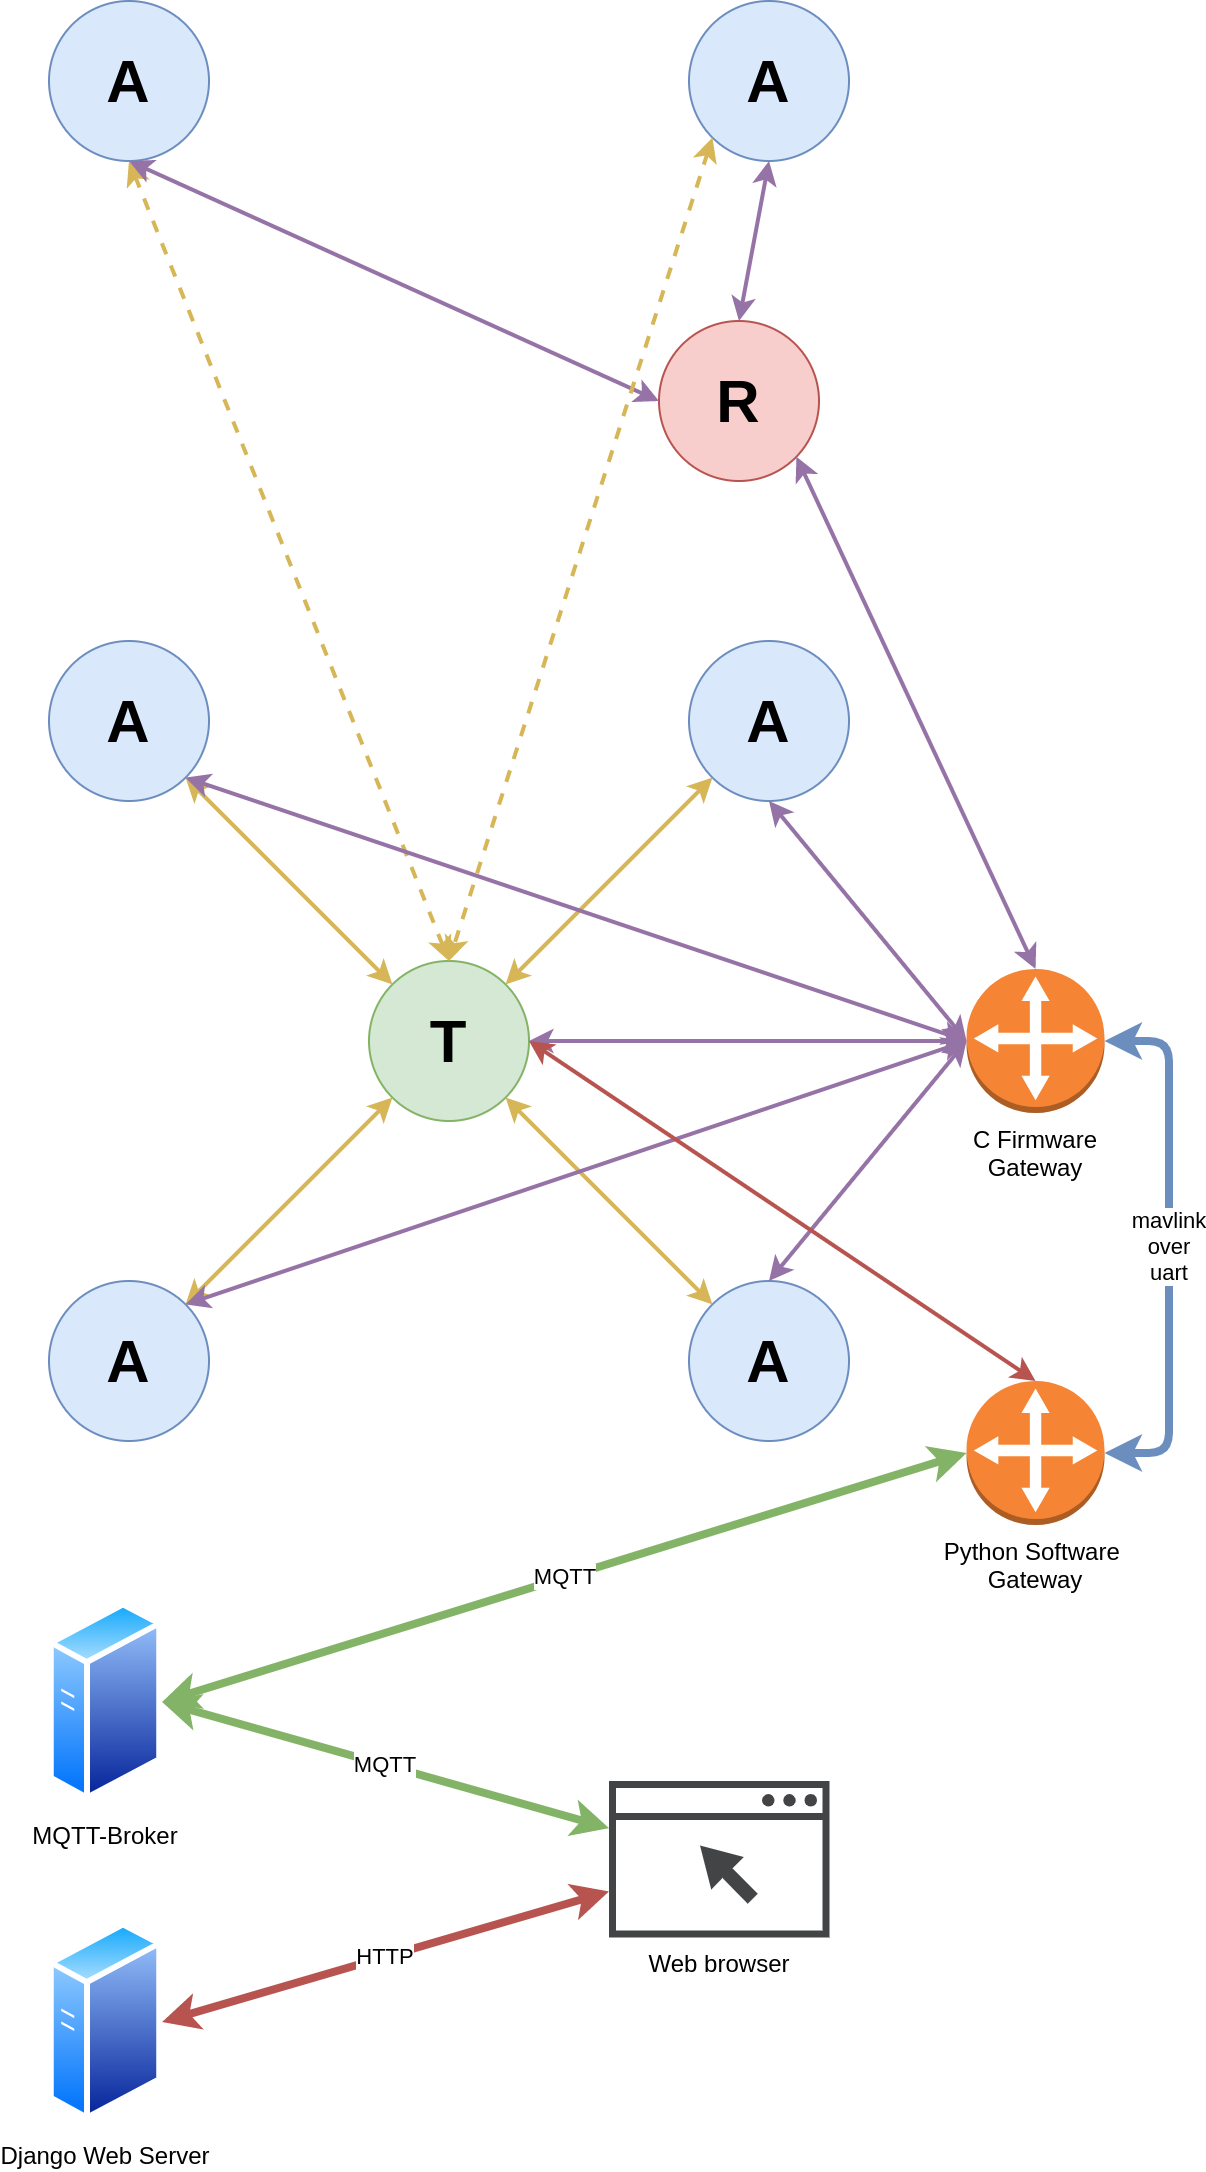
\includegraphics[width=0.9\textwidth]{system_overview.png}
    \caption{Whole system overview}
    \label{fig:system_overview}
\end{figure}
The system deployed in this thesis is illustrated in figure \ref{fig:system_overview}. There are three cells in the sample network and one tag located in each of the first two cells. Tags and anchors communicate with each other using 802.15.4 protocol over UWB radio. They, however, exchange messages with a gateway through a Bluetooth mesh network. The role of the relay node is to relay Bluetooth mesh messages as the distance between anchors/tags and gateway may longer than the effective communication range of Bluetooth-based devices. The firmware and software part of the gateway internally communicate using MAVLink protocol over a UART connection. The MAVLink frame is then stringified to JSON format and published to an MQTT broker. The control and management system is a web-based application. A Django server provides web service for this application. When receiving an HTTP request from the browser, the Django server returns an HTML/CSS-based GUI (Graphic User Interface) together with instructions for the browser to connect to the MQTT broker. In this way, the browser subscribes to the right topic. On receiving event messages from the gateway, the browser processes and shows them on the screen in a programmed way. On receiving controls from users, the browser publishes the corresponsive JSON messages to a specific topic that has been already subscribed by the gateway. The gateway then passes such messages to the mesh network.

\section{Evaluation}

In all experiments, the location error is calculated follow equation \ref{eqn:root_mean_square}.
\begin{equation}
    e_{RMS} = \frac{1}{n} \sum_{k=1}^{n} \sqrt{(x_k-x_{kg})^2 + (y_k-y_{kg})^2 + (z_k-z_{kg})^2}
    \label{eqn:root_mean_square}
\end{equation}
Where:
\begin{itemize}
    \item $e_{RMS}$ is the root mean square error;
    \item $x_k$, $y_k$, $z_k$ are the estimated coordinates of the tag at experiment $k$;
    \item $x_{gk}$, $y_{gk}$, $z_{gk}$ are the actual coordinates of the tag at experiment $k$;
\end{itemize}
The control and management interface for the experiment is shown in figure \ref{fig:result_gui}.

System performance is evaluated in 4 scenarios as provided in the following subsections.
\subsection{Scenario 1: Static Tag in Single-cell Environment}
\label{subsection:scenario_1}
\subsubsection{Objective}
The purpose of this experiment is to evaluate the accuracy of a static tag in a single cell environment.
For this purpose, a tag is placed at a number of fixed positions, this tag will then measure the distances to 4 anchors and calculate its location using the TWR method. With each position, 300 location results are obtained and the average error is calculated using equation \ref{eqn:root_mean_square}.
\subsubsection{Preparation}
Figure \ref{fig:scenario_1} illustrate the scenario used in this experiment. Four anchors are placed at the four corners of a rectangle at the height of 3 meters above the ground. A tag is placed inside the projection of the rectangle to the ground. This tag sends its calculated positions to a PCA10040-based gateway over a Bluetooth mesh network. Such results are then subscribed and processed by a computer. Figure \ref{fig:arena_00}, \ref{fig:node_0_1}, and \ref{fig:node_2_3} show the actual scenarios set up on the 3rd floor of B1 building at the Ho Chi Minh City University of Technology. Each anchor is numbered for cross-reference between figure \ref{fig:scenario_1} and \ref{fig:arena_00}.

\begin{figure}[H]   
    \centering
    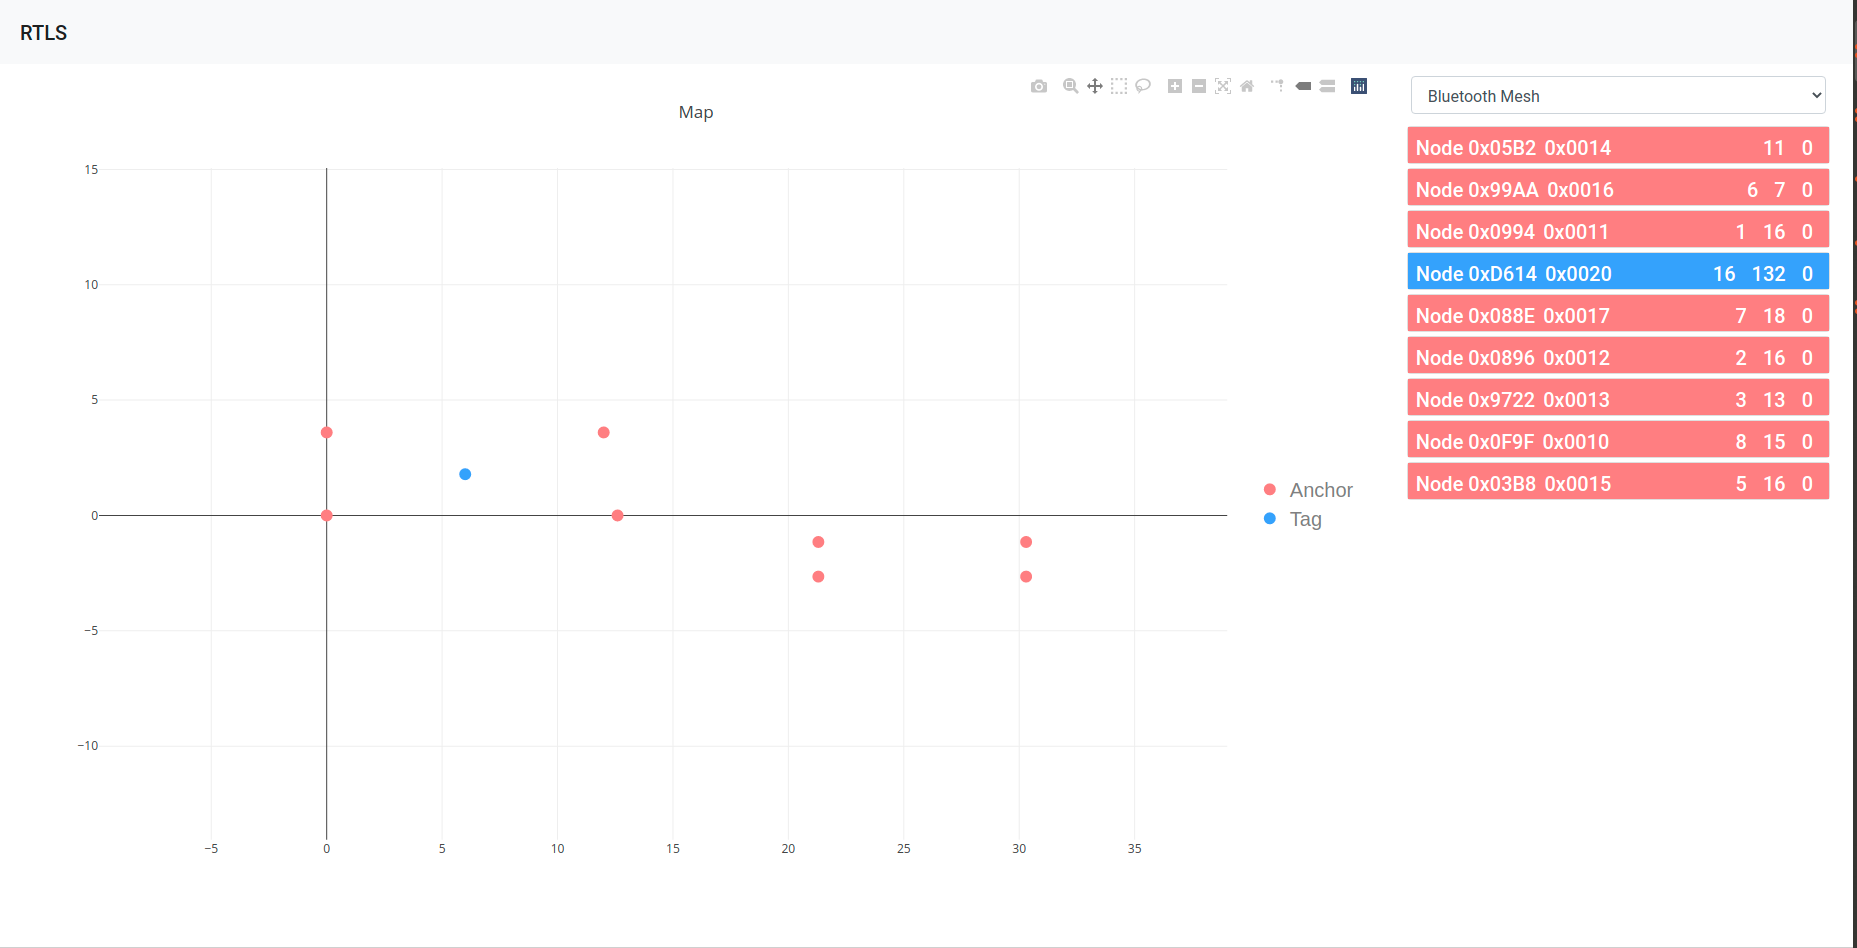
\includegraphics[angle=90, width=0.75\textwidth]{result_gui.png}
    \caption{GUI for the IPS}
    \label{fig:result_gui}
\end{figure}

 
\begin{figure}[H]
    \centering
    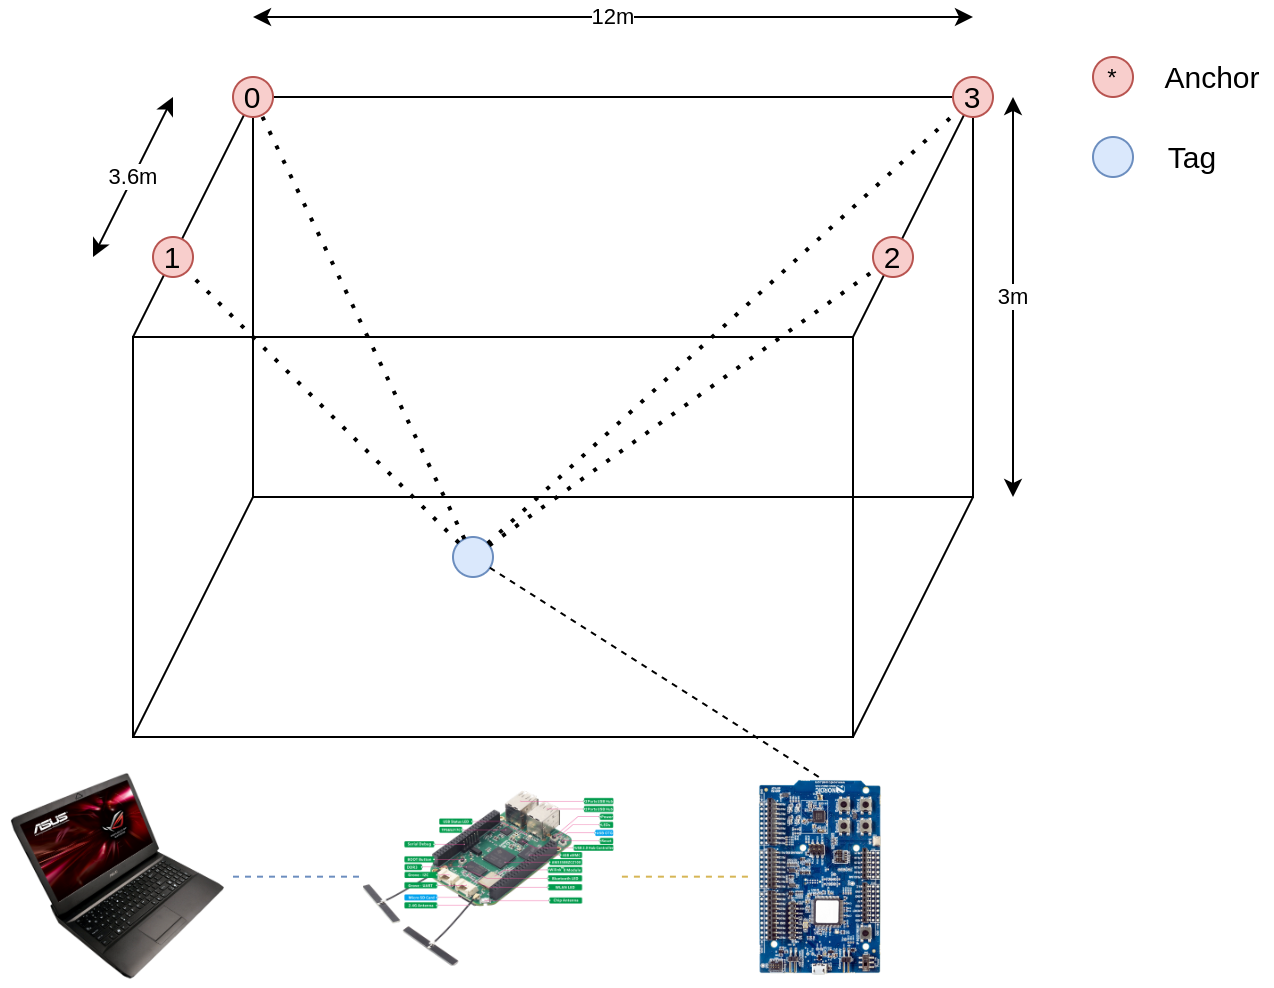
\includegraphics[width=0.8\textwidth]{system_overview_phy.png}
    \caption{Scenario 1}
    \label{fig:scenario_1}
\end{figure}

\begin{figure}[H]      
    \centering
    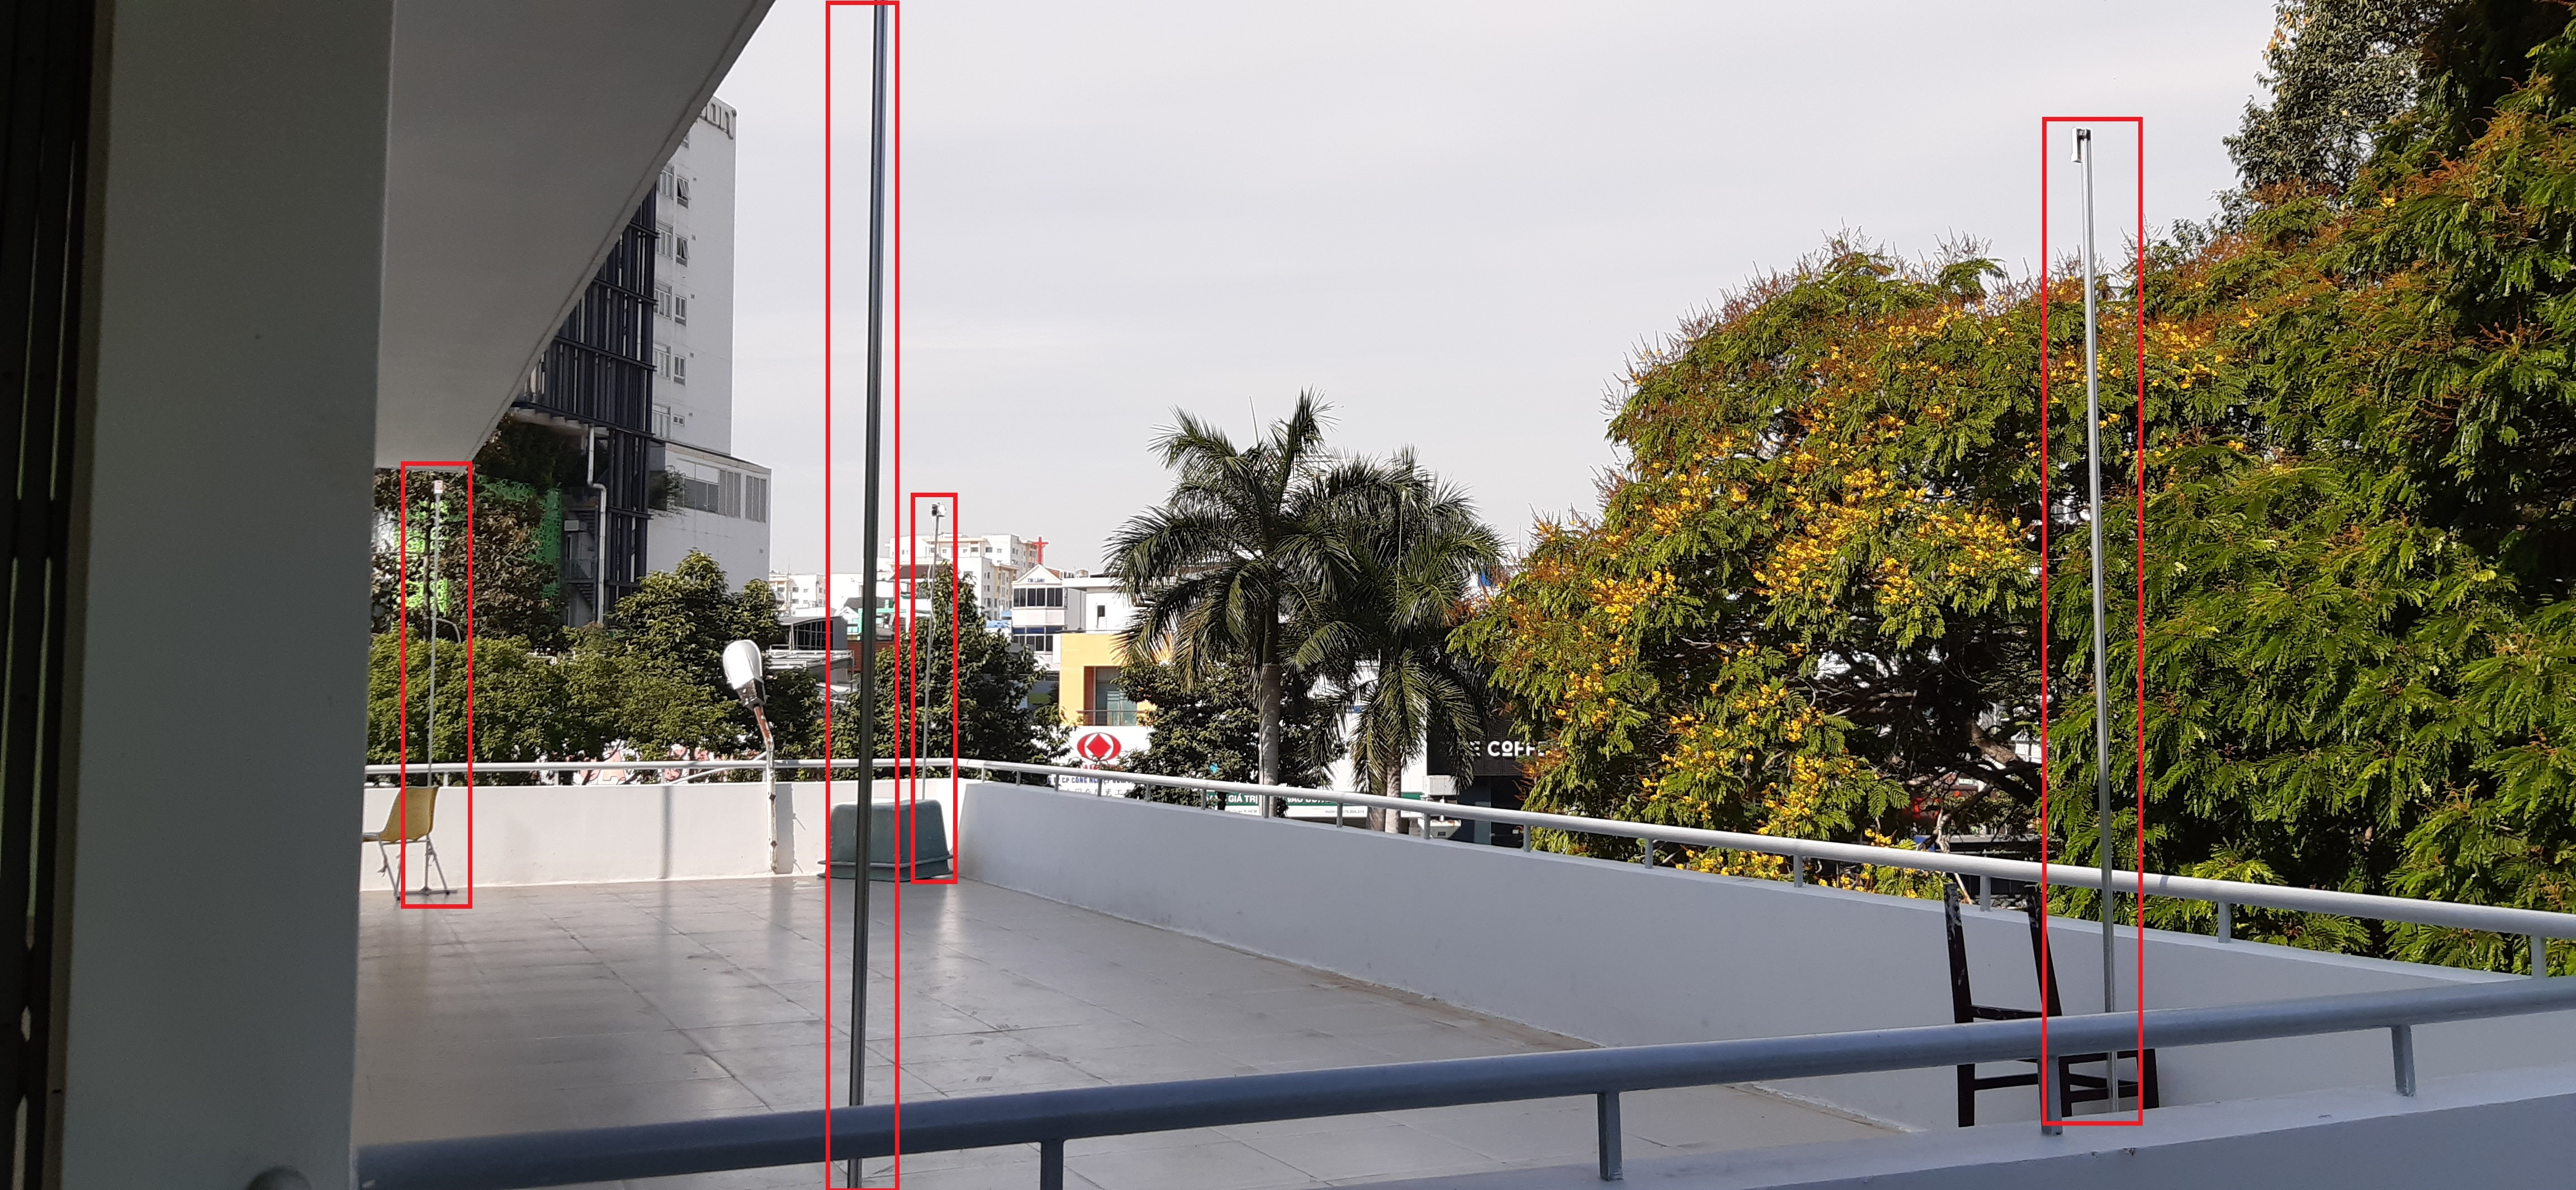
\includegraphics[width=1\textwidth]{arena_00.jpg}
    \caption{Arena side view}
    \label{fig:arena_00}
\end{figure}

\begin{figure}[H]      
    \centering
    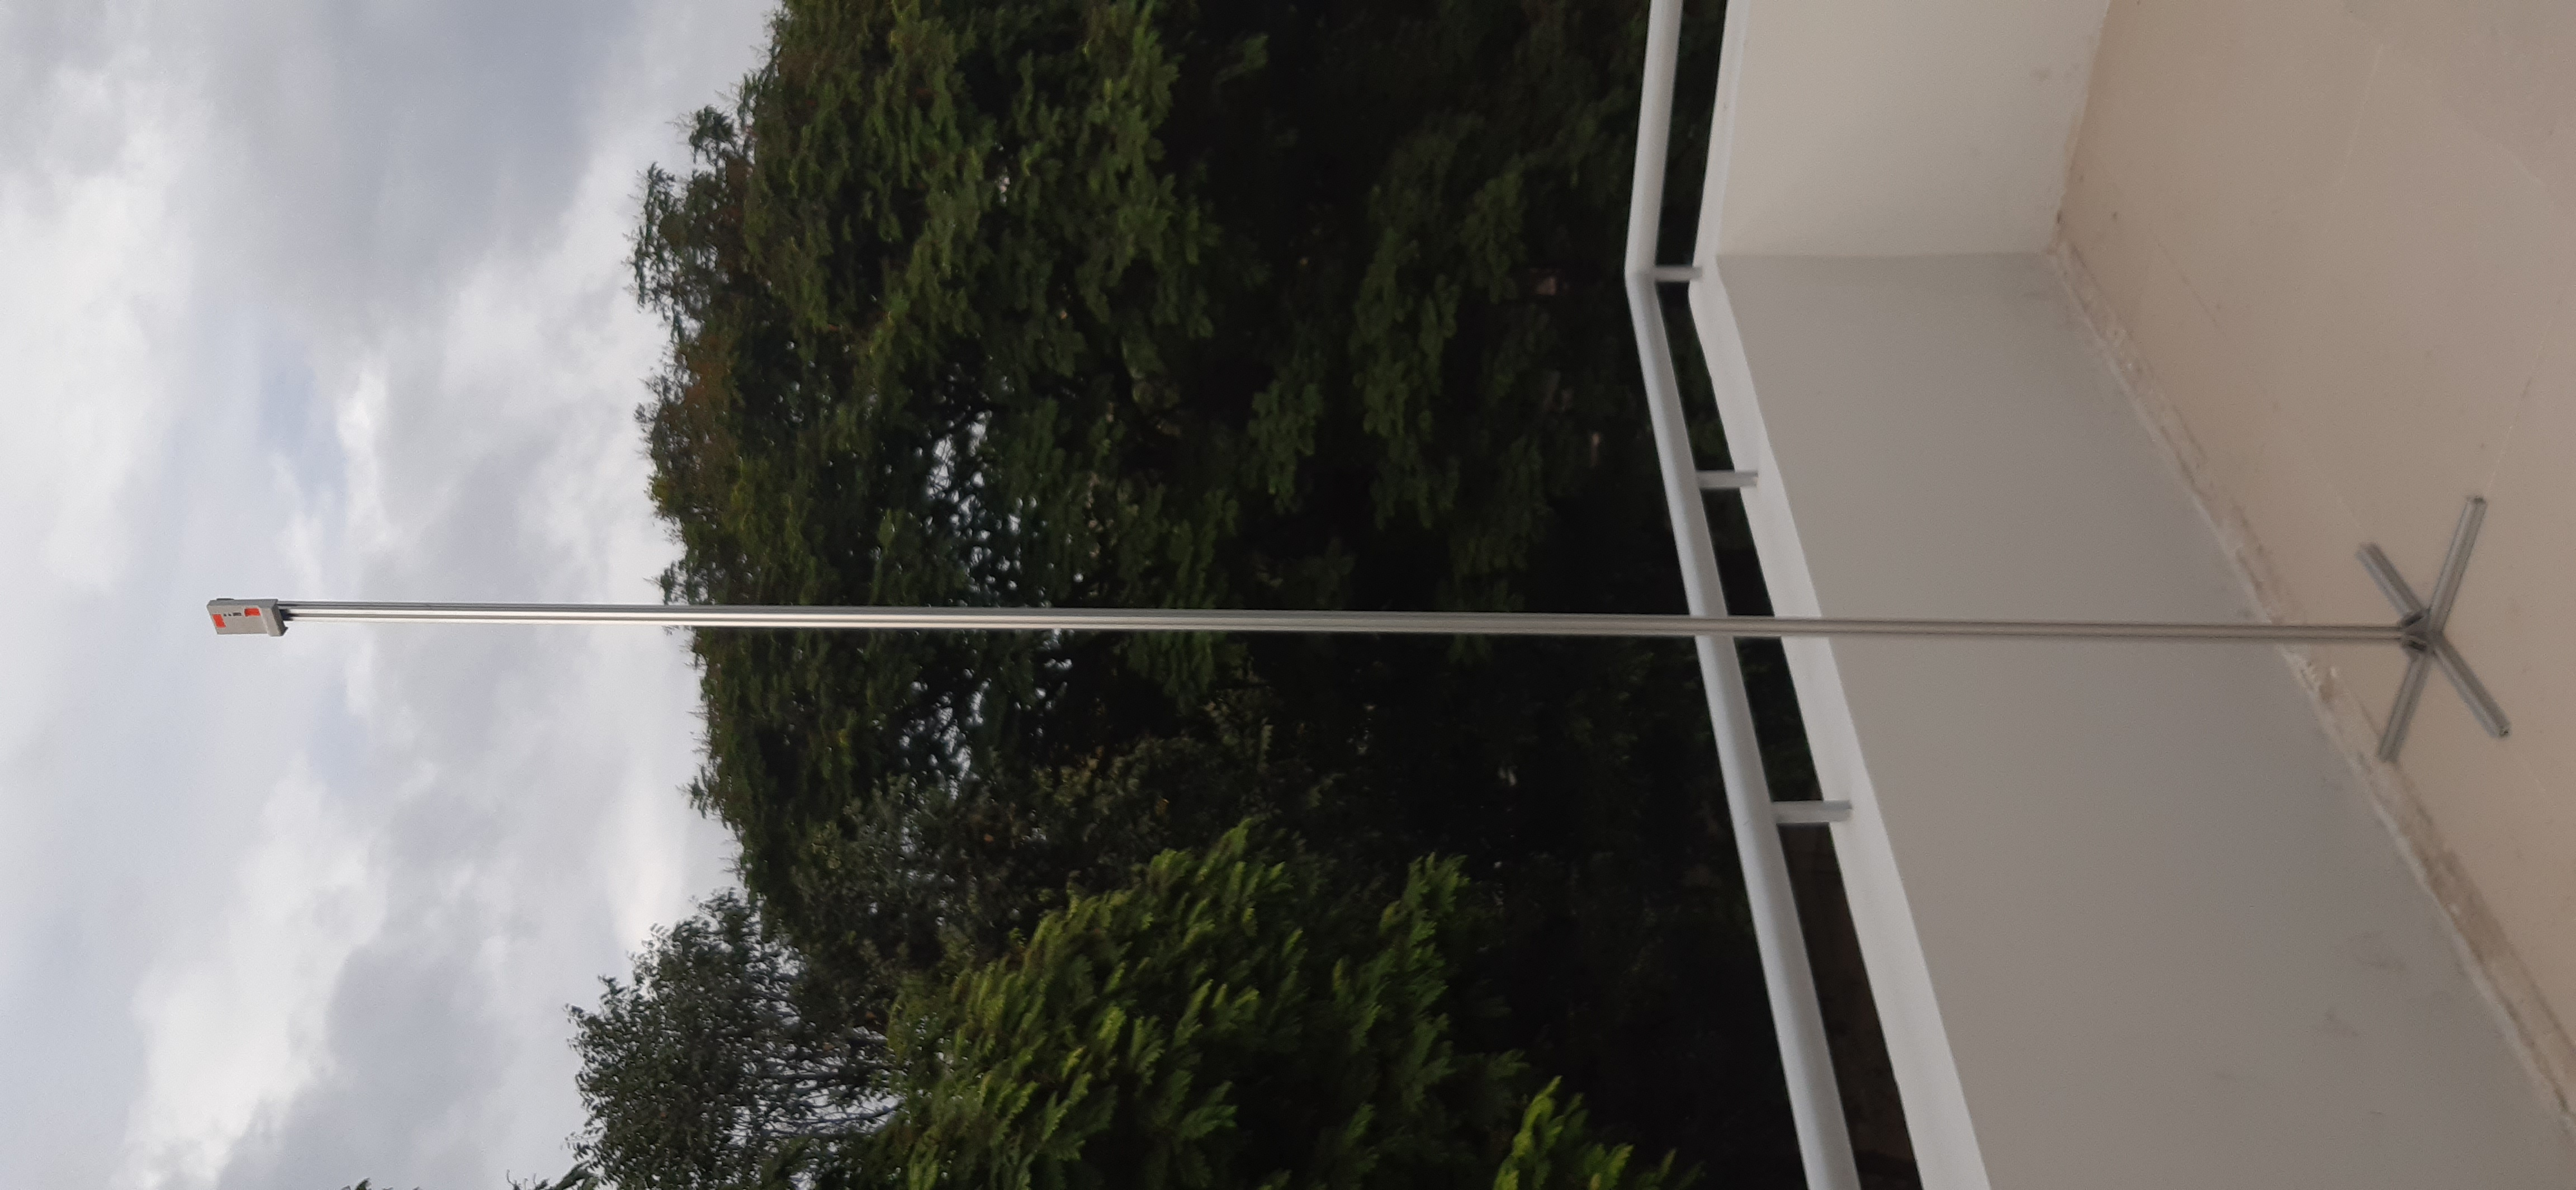
\includegraphics[width=1\textwidth]{arena_01.jpg}
    \caption{Node 0,1}
    \label{fig:node_0_1}
\end{figure}

\begin{figure}[H]      
    \centering
    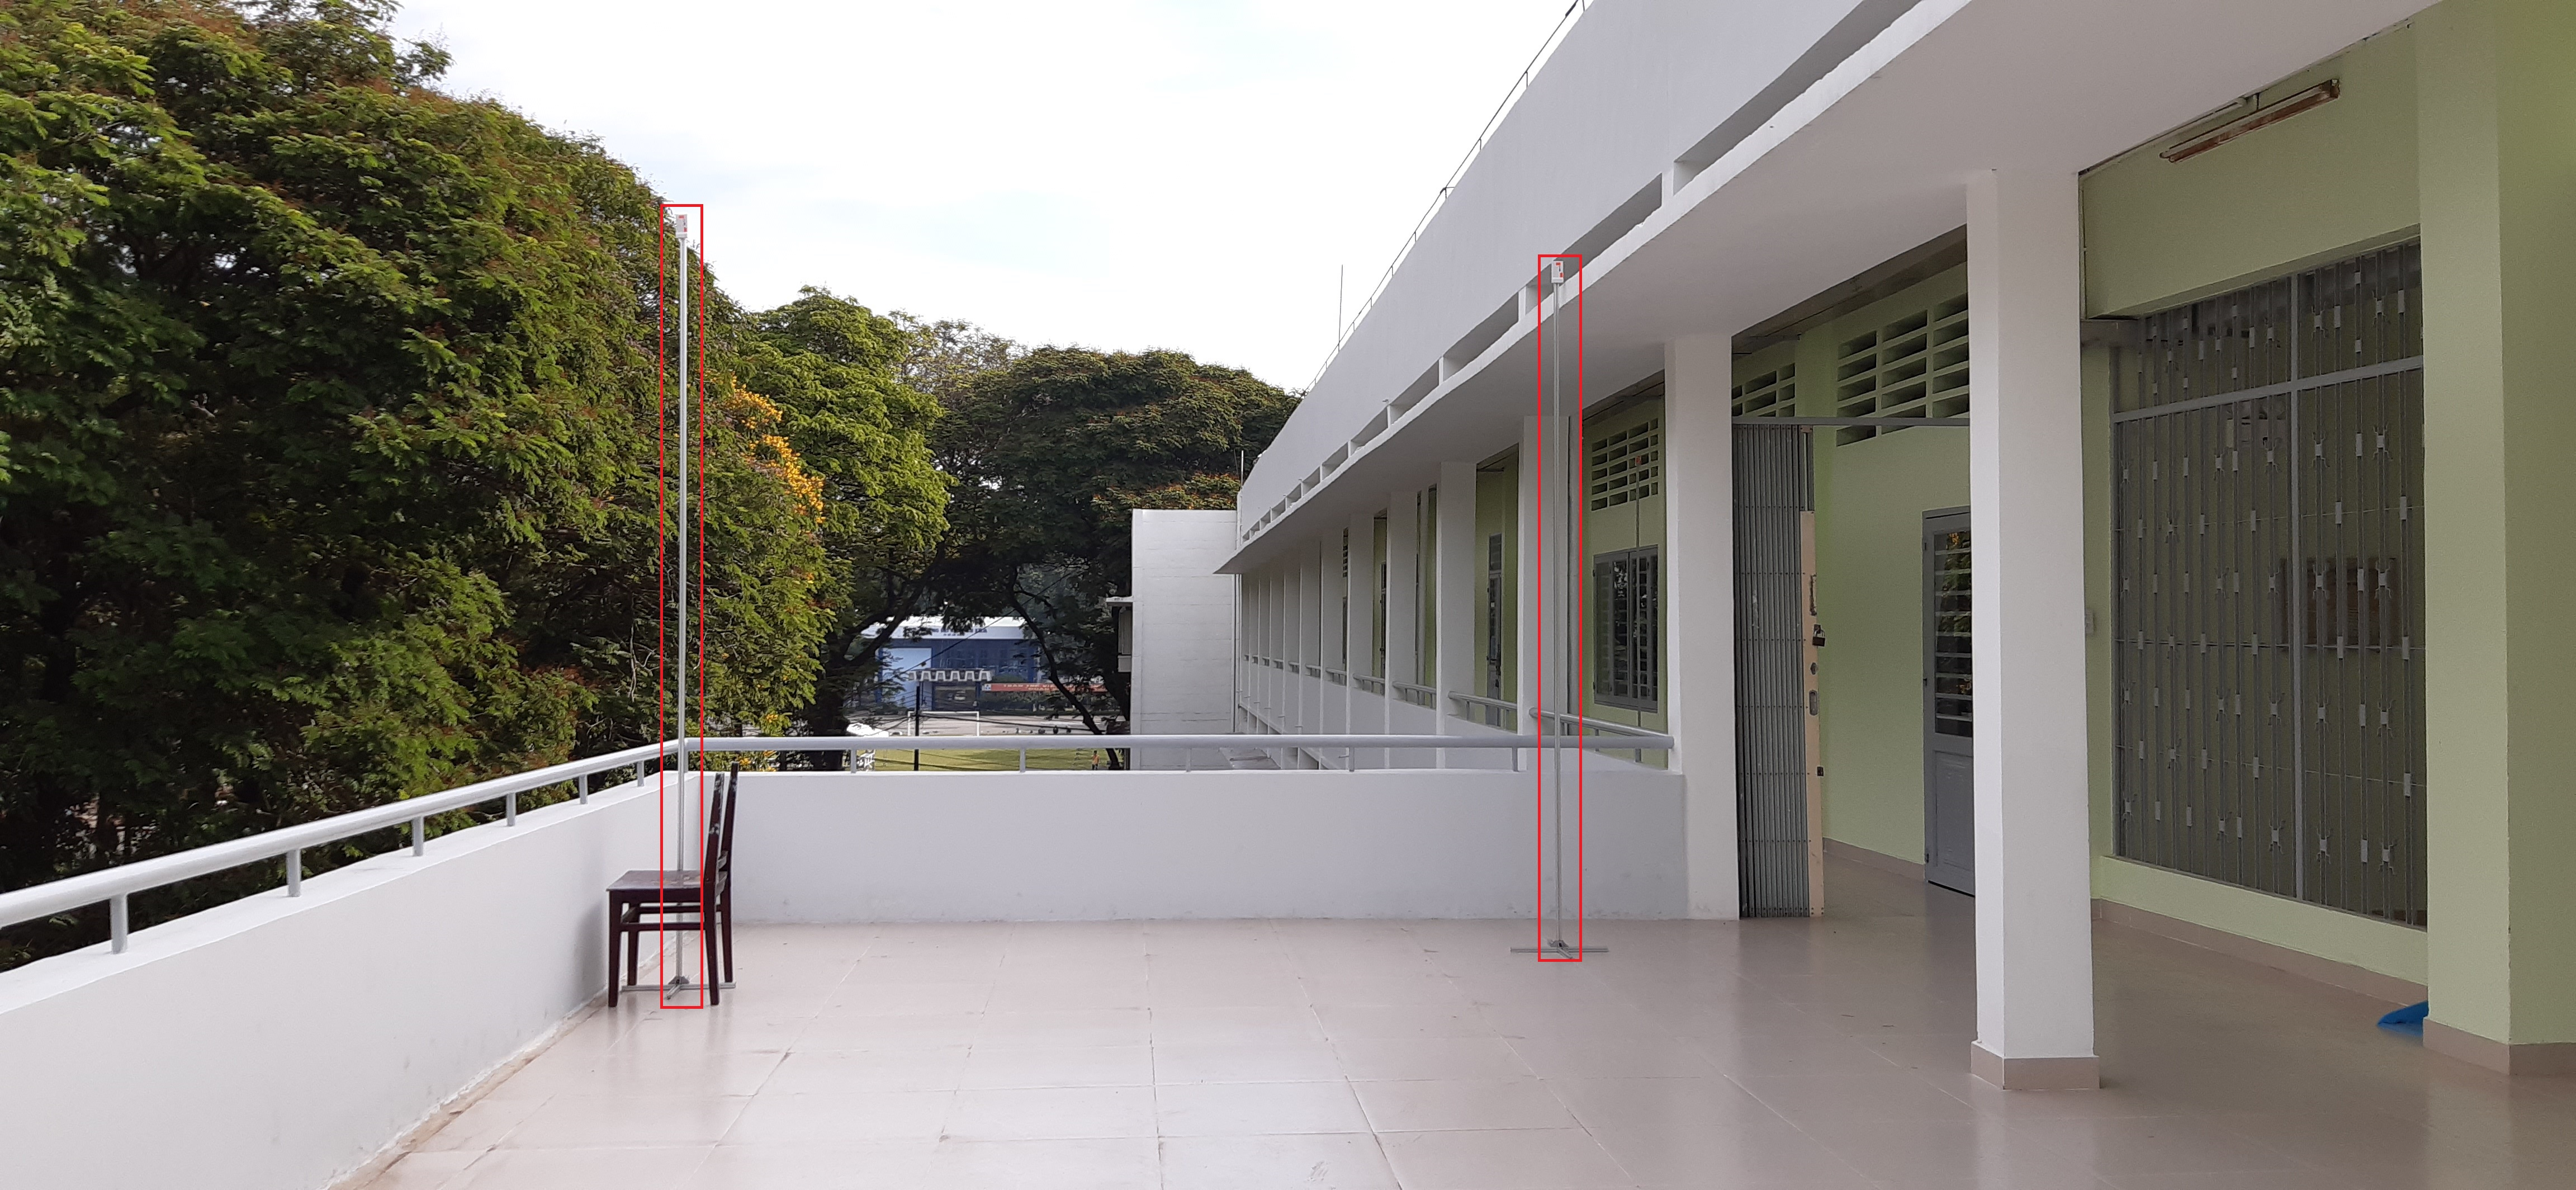
\includegraphics[width=1\textwidth]{arena_02.jpg}
    \caption{Node 2,3}
    \label{fig:node_2_3}
\end{figure}

\subsubsection{Result}

Table \ref{table:vendor_rms_error} and \ref{table:proposed_rms_error} provide RMS errors of the vendor reference and proposed system relative to the position $(x,y)$. Figure \ref{fig:vendor_rms_error} and \ref{fig:proposed_rms_error} graphically illustrate the error. In such figures, blue points show the reference location and red circles illustrate mean error for each of these locations.

\begin{table}[ht]
    \centering
    \begin{tabular}{|c|>{\centering\arraybackslash}p{2cm}|>{\centering\arraybackslash}p{2cm}|>{\centering\arraybackslash}p{2cm}|}
    \hline
    \backslashbox{y(m)}{x(m)}  &  3 & 7 & 10 \\ \hline
    0 &  0.2 &  0.28 &  0.25  \\ \hline
    2 &  0.14 &  0.13 &  0.18  \\ \hline
    4 &  0.22 &  0.19 &  0.27  \\ \hline
    \end{tabular}
    \caption{Vendor system error}
    \label{table:vendor_rms_error}
\end{table}

\begin{table}[H]
    \centering
    \begin{tabular}{|c|>{\centering\arraybackslash}p{2cm}|>{\centering\arraybackslash}p{2cm}|>{\centering\arraybackslash}p{2cm}|>{\centering\arraybackslash}p{2cm}|}
    \hline
    \backslashbox{y(m)}{x(m)}  &  1.2 & 4.8 & 9.6 & 10.8 \\ \hline
    0.6 &  0.10 & 0.20&  0.13 &  0.12  \\ \hline
    1.2 &  0.13 & 0.18&  0.17 &  0.16  \\ \hline
    2.4 &  0.09 & 0.10&  0.11 &  0.22  \\ \hline
    \end{tabular}
    \caption{Proposed system error}
    \label{table:proposed_rms_error}
\end{table}

\begin{figure}[H]
    \begin{minipage}[t]{\textwidth}       
        \centering
        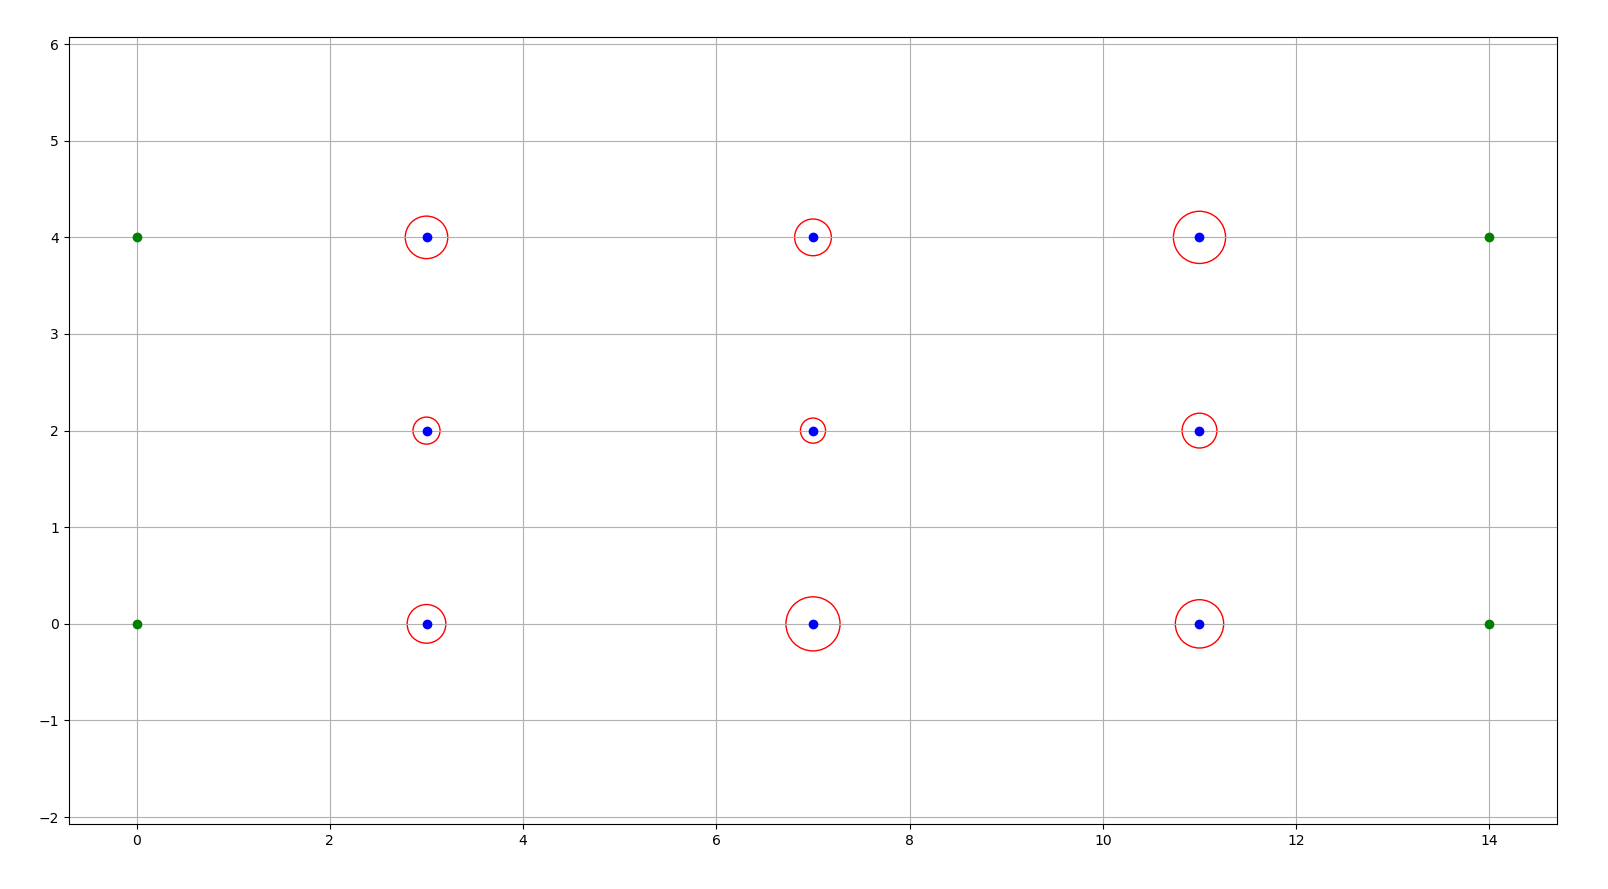
\includegraphics[width=1\textwidth]{rms_error}
    \end{minipage}
    \caption{Vendor system error}
    \label{fig:vendor_rms_error}
\end{figure}

\begin{figure}[H]     
    \centering
    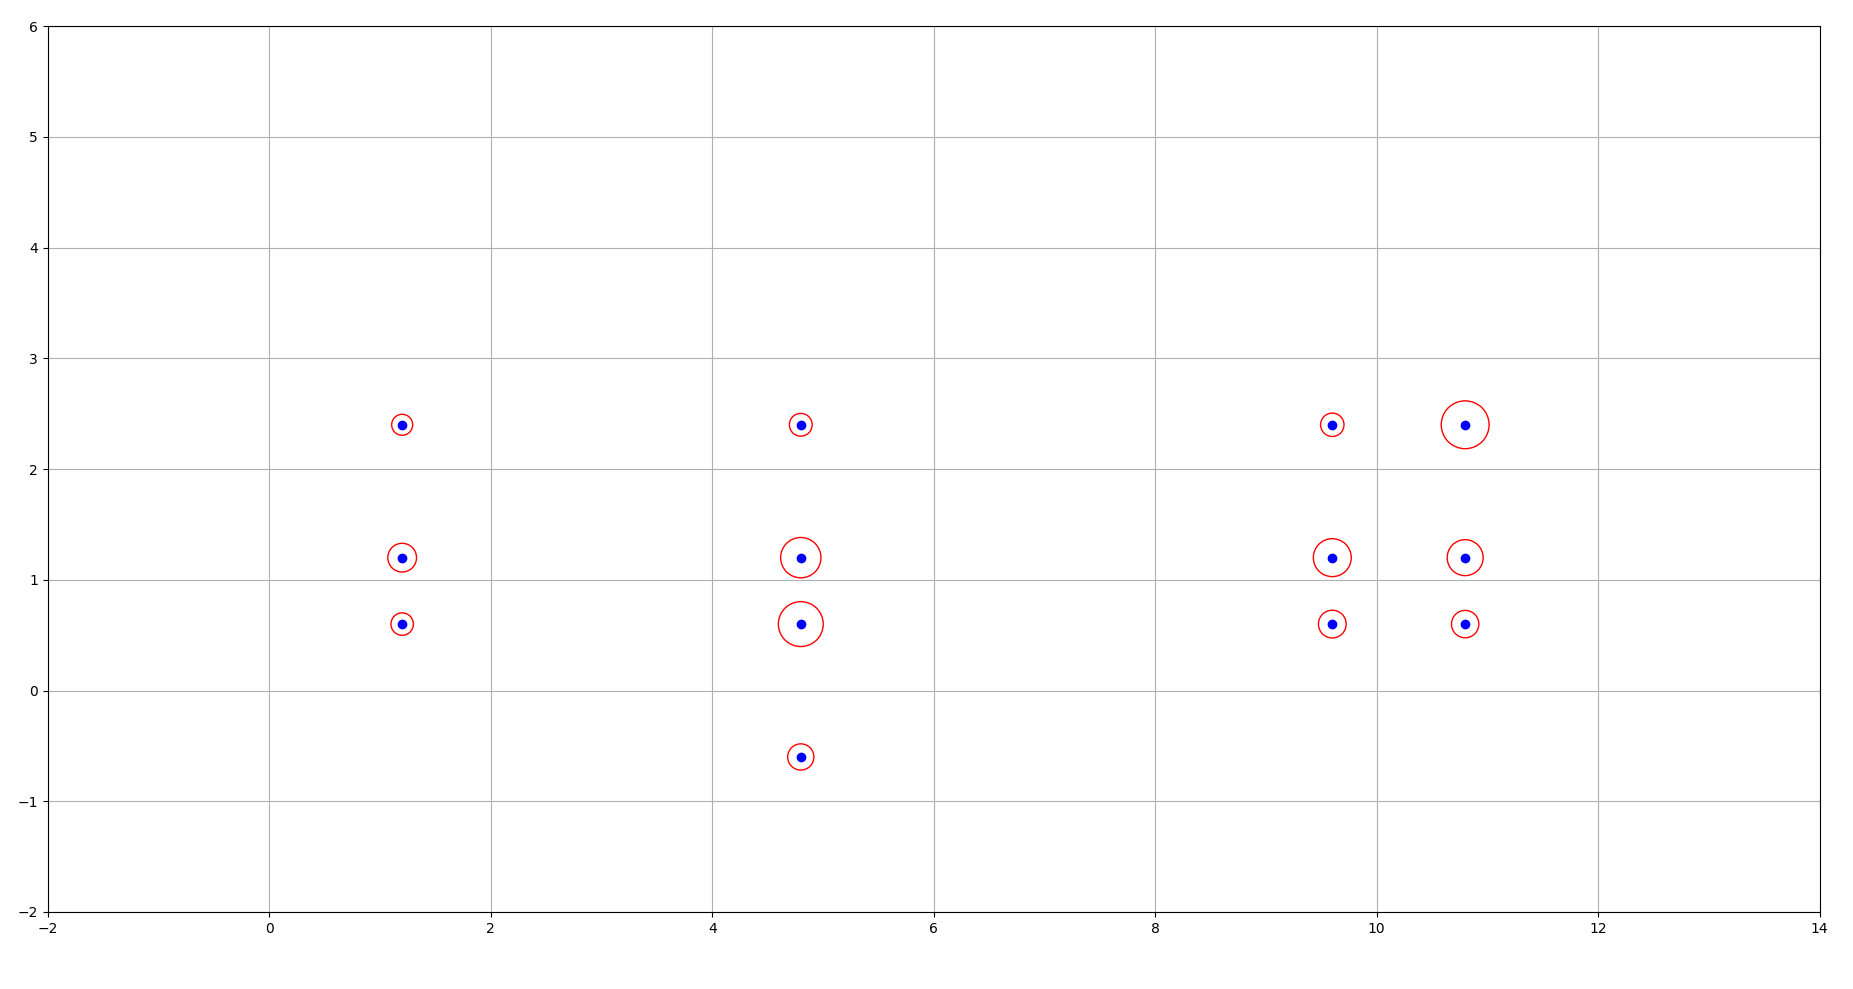
\includegraphics[width=1\textwidth]{result_static.png}
    \caption{Proposed system error}
    \label{fig:proposed_rms_error}
\end{figure}

% \subsection{Preparation}
% This subsection provides images to illustrate the experimental setup used to evaluate the proposed localization system. The logical configuration of the system has been given in figure \ref{fig:system_overview}. The physical placement of devices is represented in figure \ref{fig:physical placement of devices}.

\subsubsection{Evaluation}
From experimental results shown in table \ref{table:vendor_rms_error} and \ref{table:proposed_rms_error}, we conclude that the proposed system has a similar performance to the reference system given by the DecaWave.
%  while provides a better IoT service (Bluetooth mesh instead of normal Bluetooth Low Energy) which reduce the price of the entire system.

\subsection{Scenario 2: Mobile Tag in Single-cell Environment}

\subsubsection{Objective}
The only purpose is to give an intuitive performance evaluation of the system when a tag moves along a specific path in a single cell.
\subsubsection{Preparation}
This experiment is set up similarly with subsection \ref{subsection:scenario_1}.
\subsubsection{Result}

Results shown in figure \ref{fig:result_rectangle} are obtained as a tag moves along the boundary of a rectangle. Since the reference path is not accurate enough, a numeric error is not provided. Notice that red lines are the reference path and blue dots are estimated positions as the tag move along the path.

\begin{figure}[H]
    \centering
    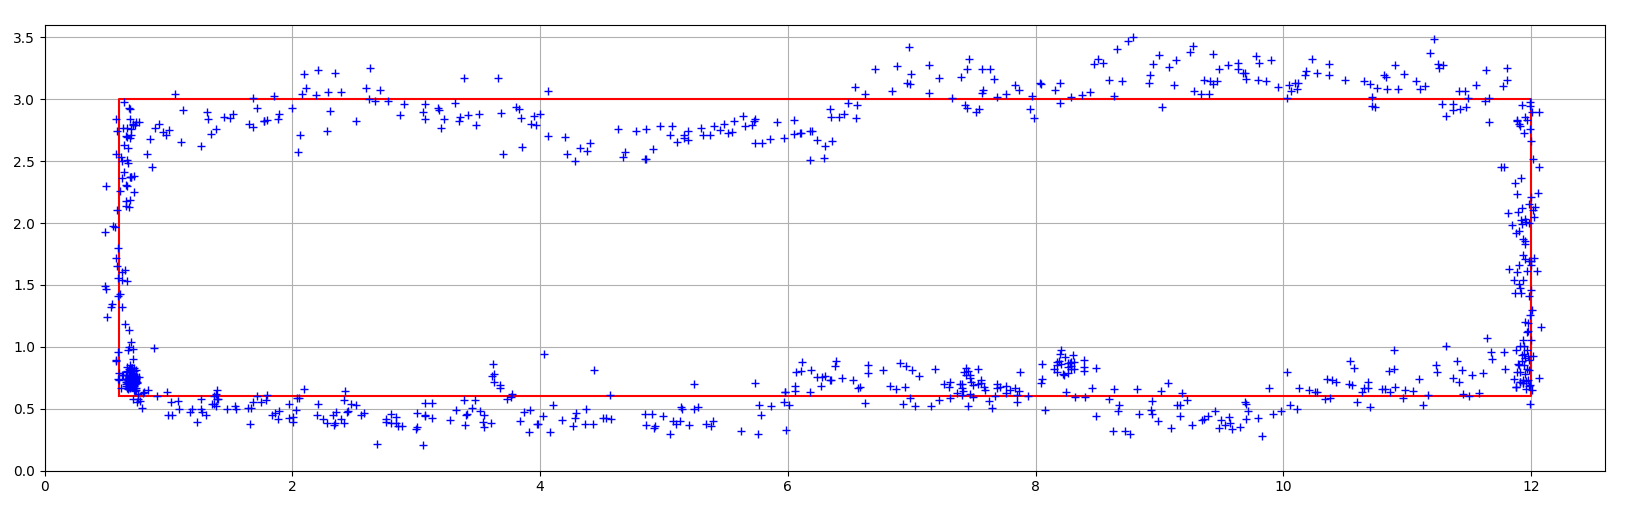
\includegraphics[width=1\textwidth]{result_square.png}
    \caption{Rectangle movement result}
    \label{fig:result_rectangle}
\end{figure}

\subsubsection{Evaluation}

For a mobile tag, the system performance is relatively low compared with a static one. However, this may be acceptable for simple applications.

% The actual placement of devices is shown in figures: \ref{fig:arena_00}, \ref{fig:node_0_1}, \ref{fig:node_2_3}, \ref{fig:node_4_5_6_7}.

\subsection{Scenario 3: Mobile Tag in Multi-cell Environment}

\subsubsection{Objective}
The goal of this experiment is to give an intuitive performance evaluation of the system when a tag moves along a specific path in a multi-cell environment.
\subsubsection{Preparation}
% This experiment is set up similarly with subsection \ref{subsection:scenario_1}.
% The scenario used in this evaluation is illustrated in figure \ref{fig:scenario_3}
In this scenario, four anchors are added to form three cells topology as illustrated in figure \ref{fig:scenario_3}. The first cell contains 4 anchors: 0, 1, 2, 3; the second cell contains 4 anchors: 2, 3, 4, 5 and the last cell contains 4 anchors: 4, 5, 6, 7. Moreover, a new PCA10040 board is added to relay Bluetooth mesh messages as the tag is now able to move away from the gateway that makes it impossible to transfer messages over a single-hope connection. The actual placement of anchors added in this experiment is shown in figure \ref{fig:node_4_5_6_7}.
Similar to subsection \ref{subsection:scenario_1}, all anchors are numbered for cross-reference purpose.
\begin{figure}[H]   
    \centering
    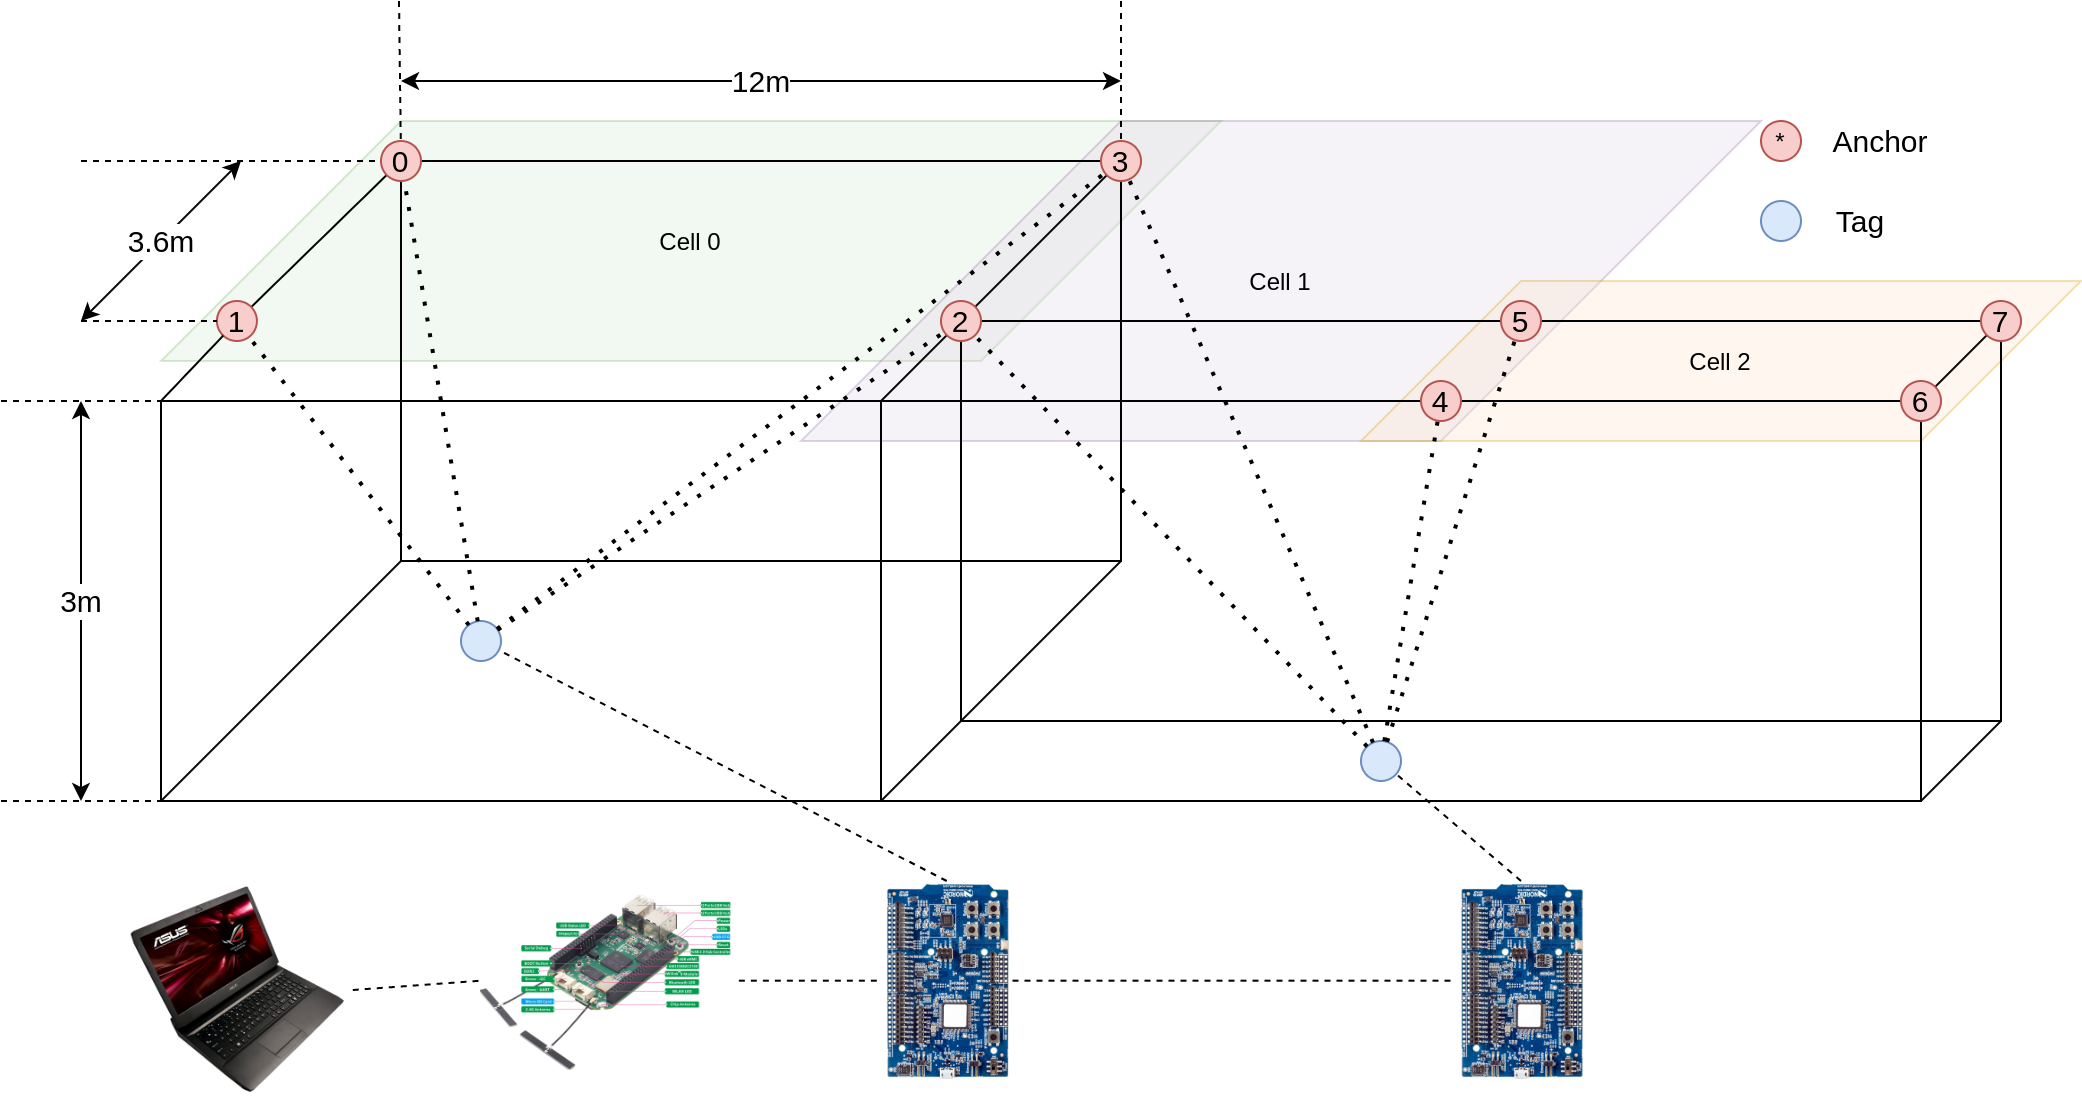
\includegraphics[width=1\textwidth]{system_overview_phy_full.png}
    \caption{Scenario 3}
    \label{fig:scenario_3}
\end{figure}
\begin{figure}[H]      
    \centering
    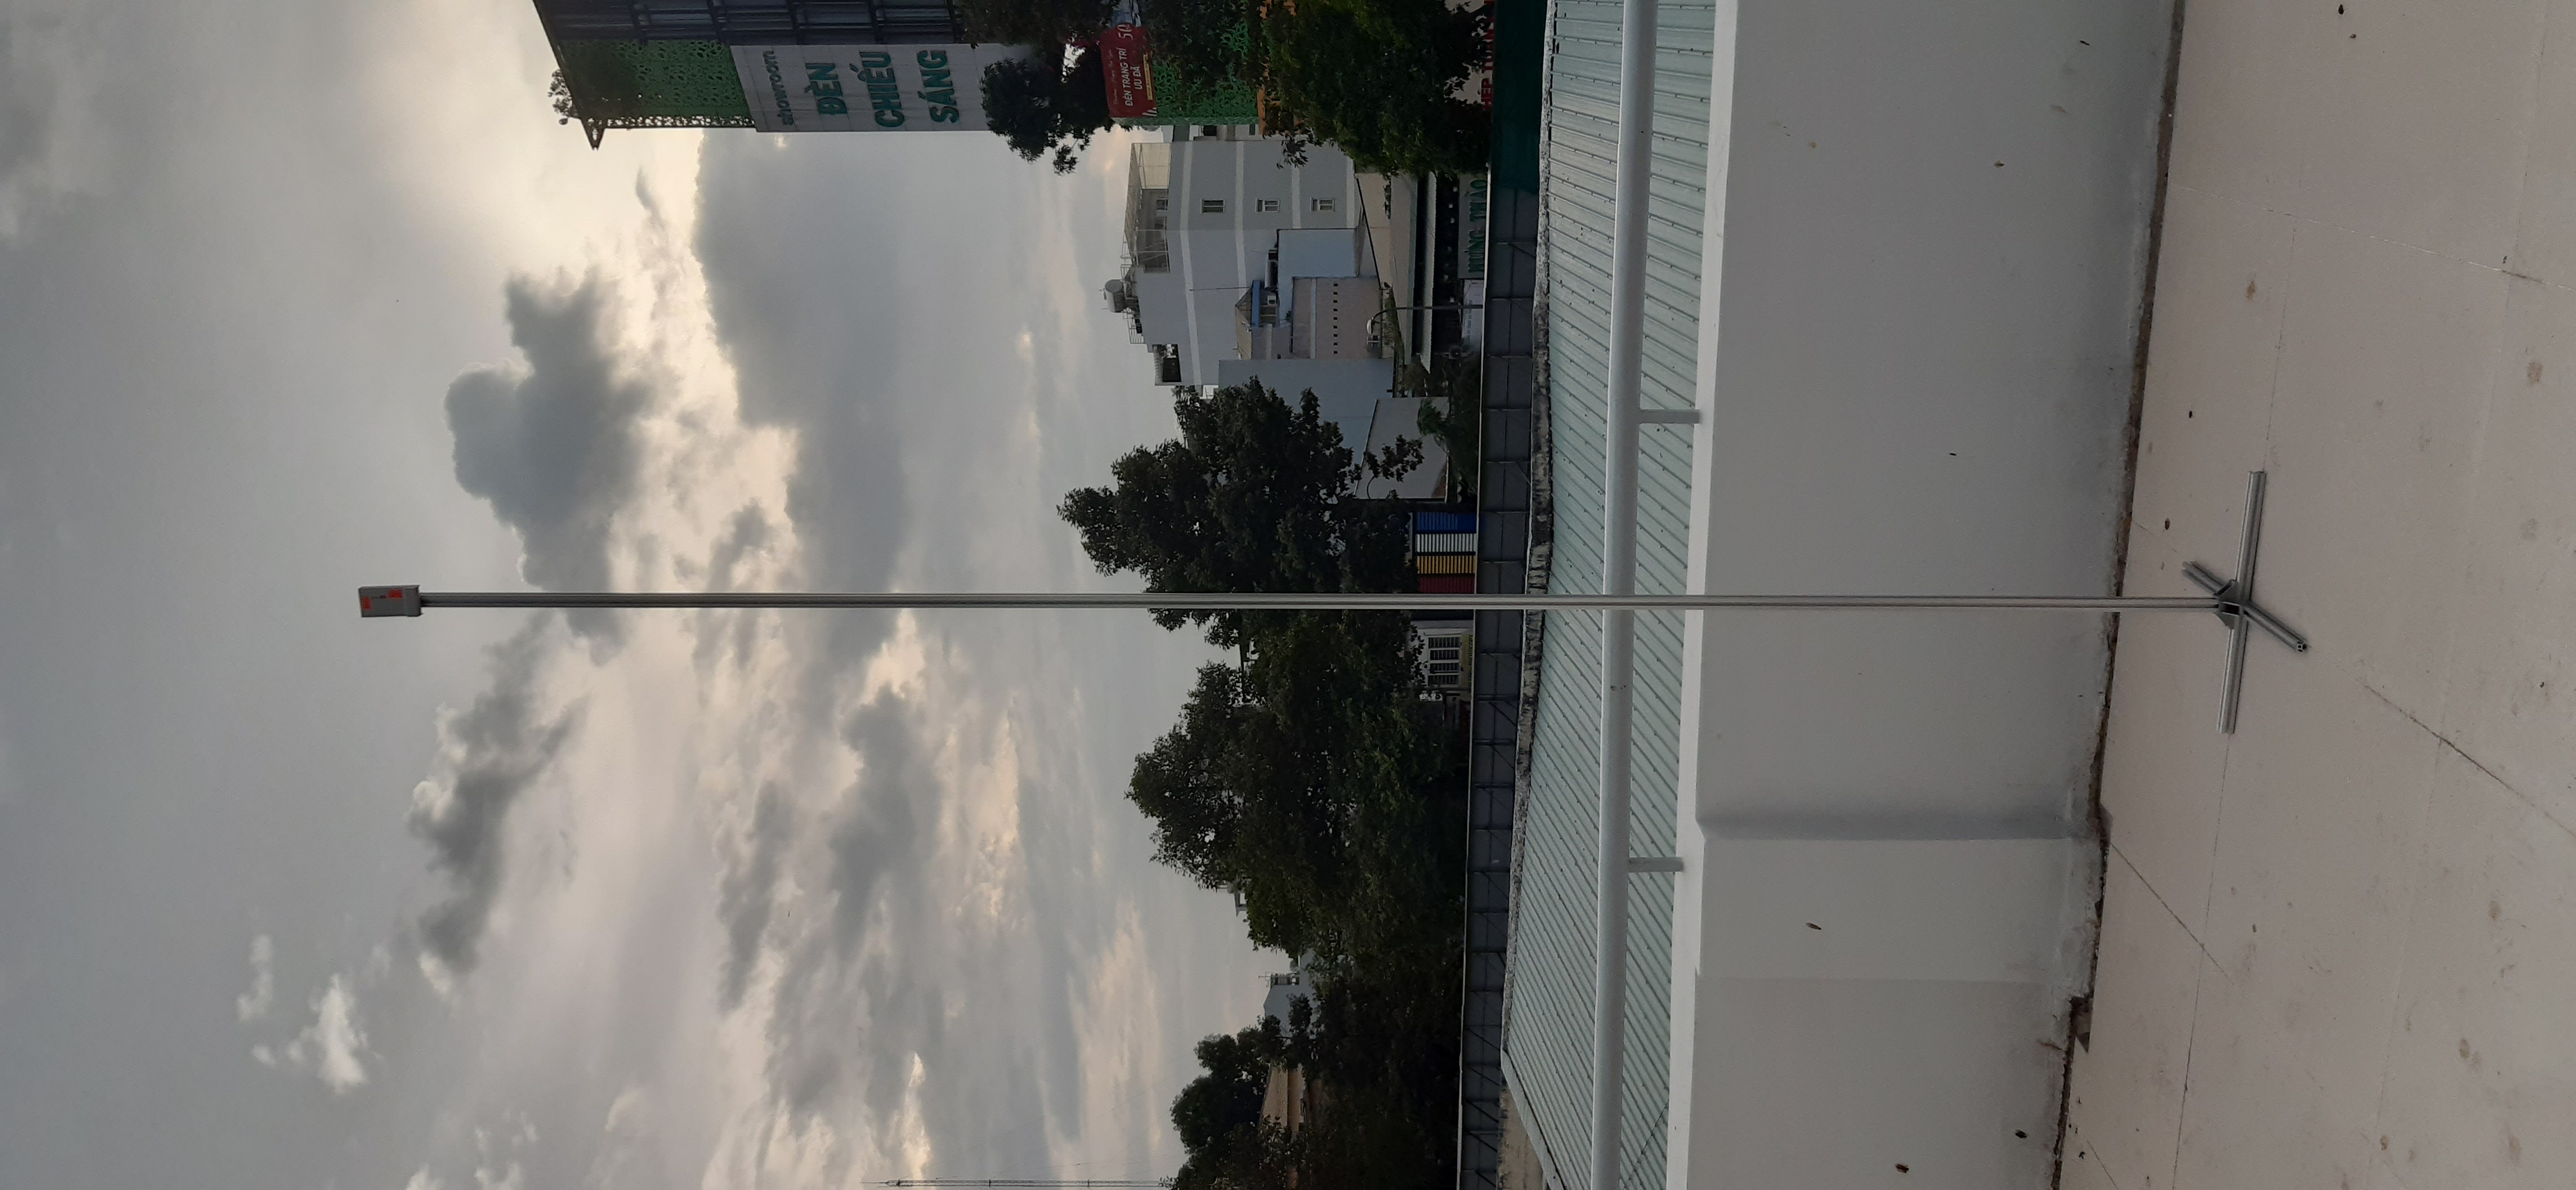
\includegraphics[width=1\textwidth]{arena_03.jpg}
    \caption{Node 4,5,6,7}
    \label{fig:node_4_5_6_7}
\end{figure}
\subsubsection{Result}
% \begin{figure}[H]
%     \centering
%     \begin{subfigure}[b]{0.4\linewidth}
%         \centering
%         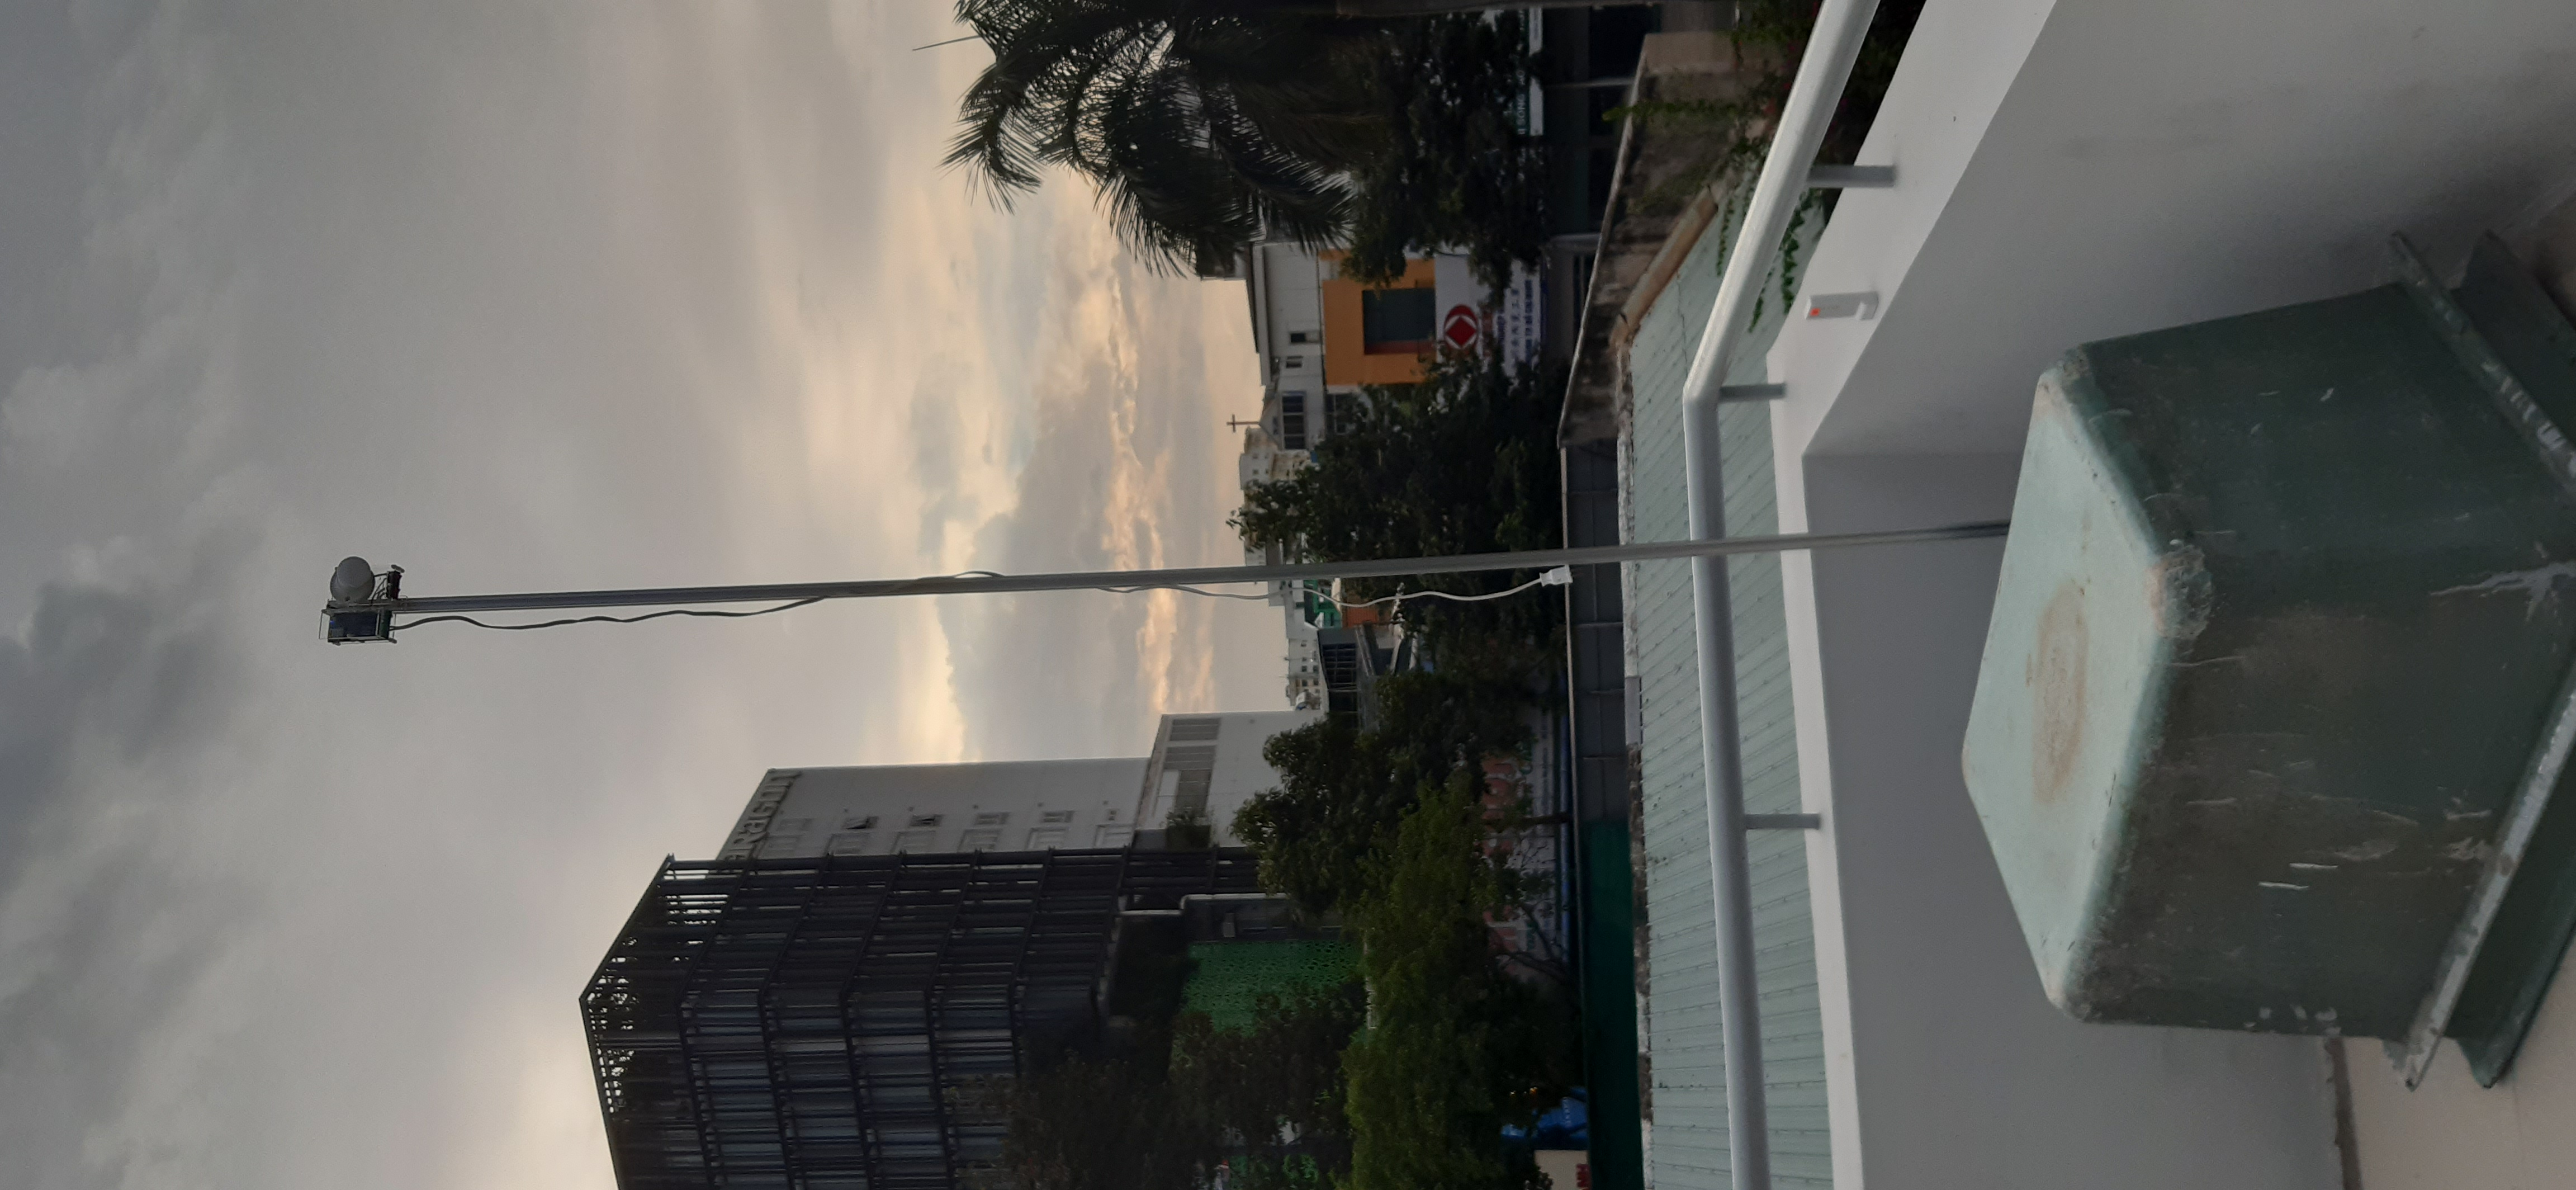
\includegraphics[angle=-90, width=0.65\linewidth]{arena_04.jpg}
%         \label{fig:arena_04}
%     \end{subfigure}
%     \begin{subfigure}[b]{0.4\linewidth}
%         \centering
%         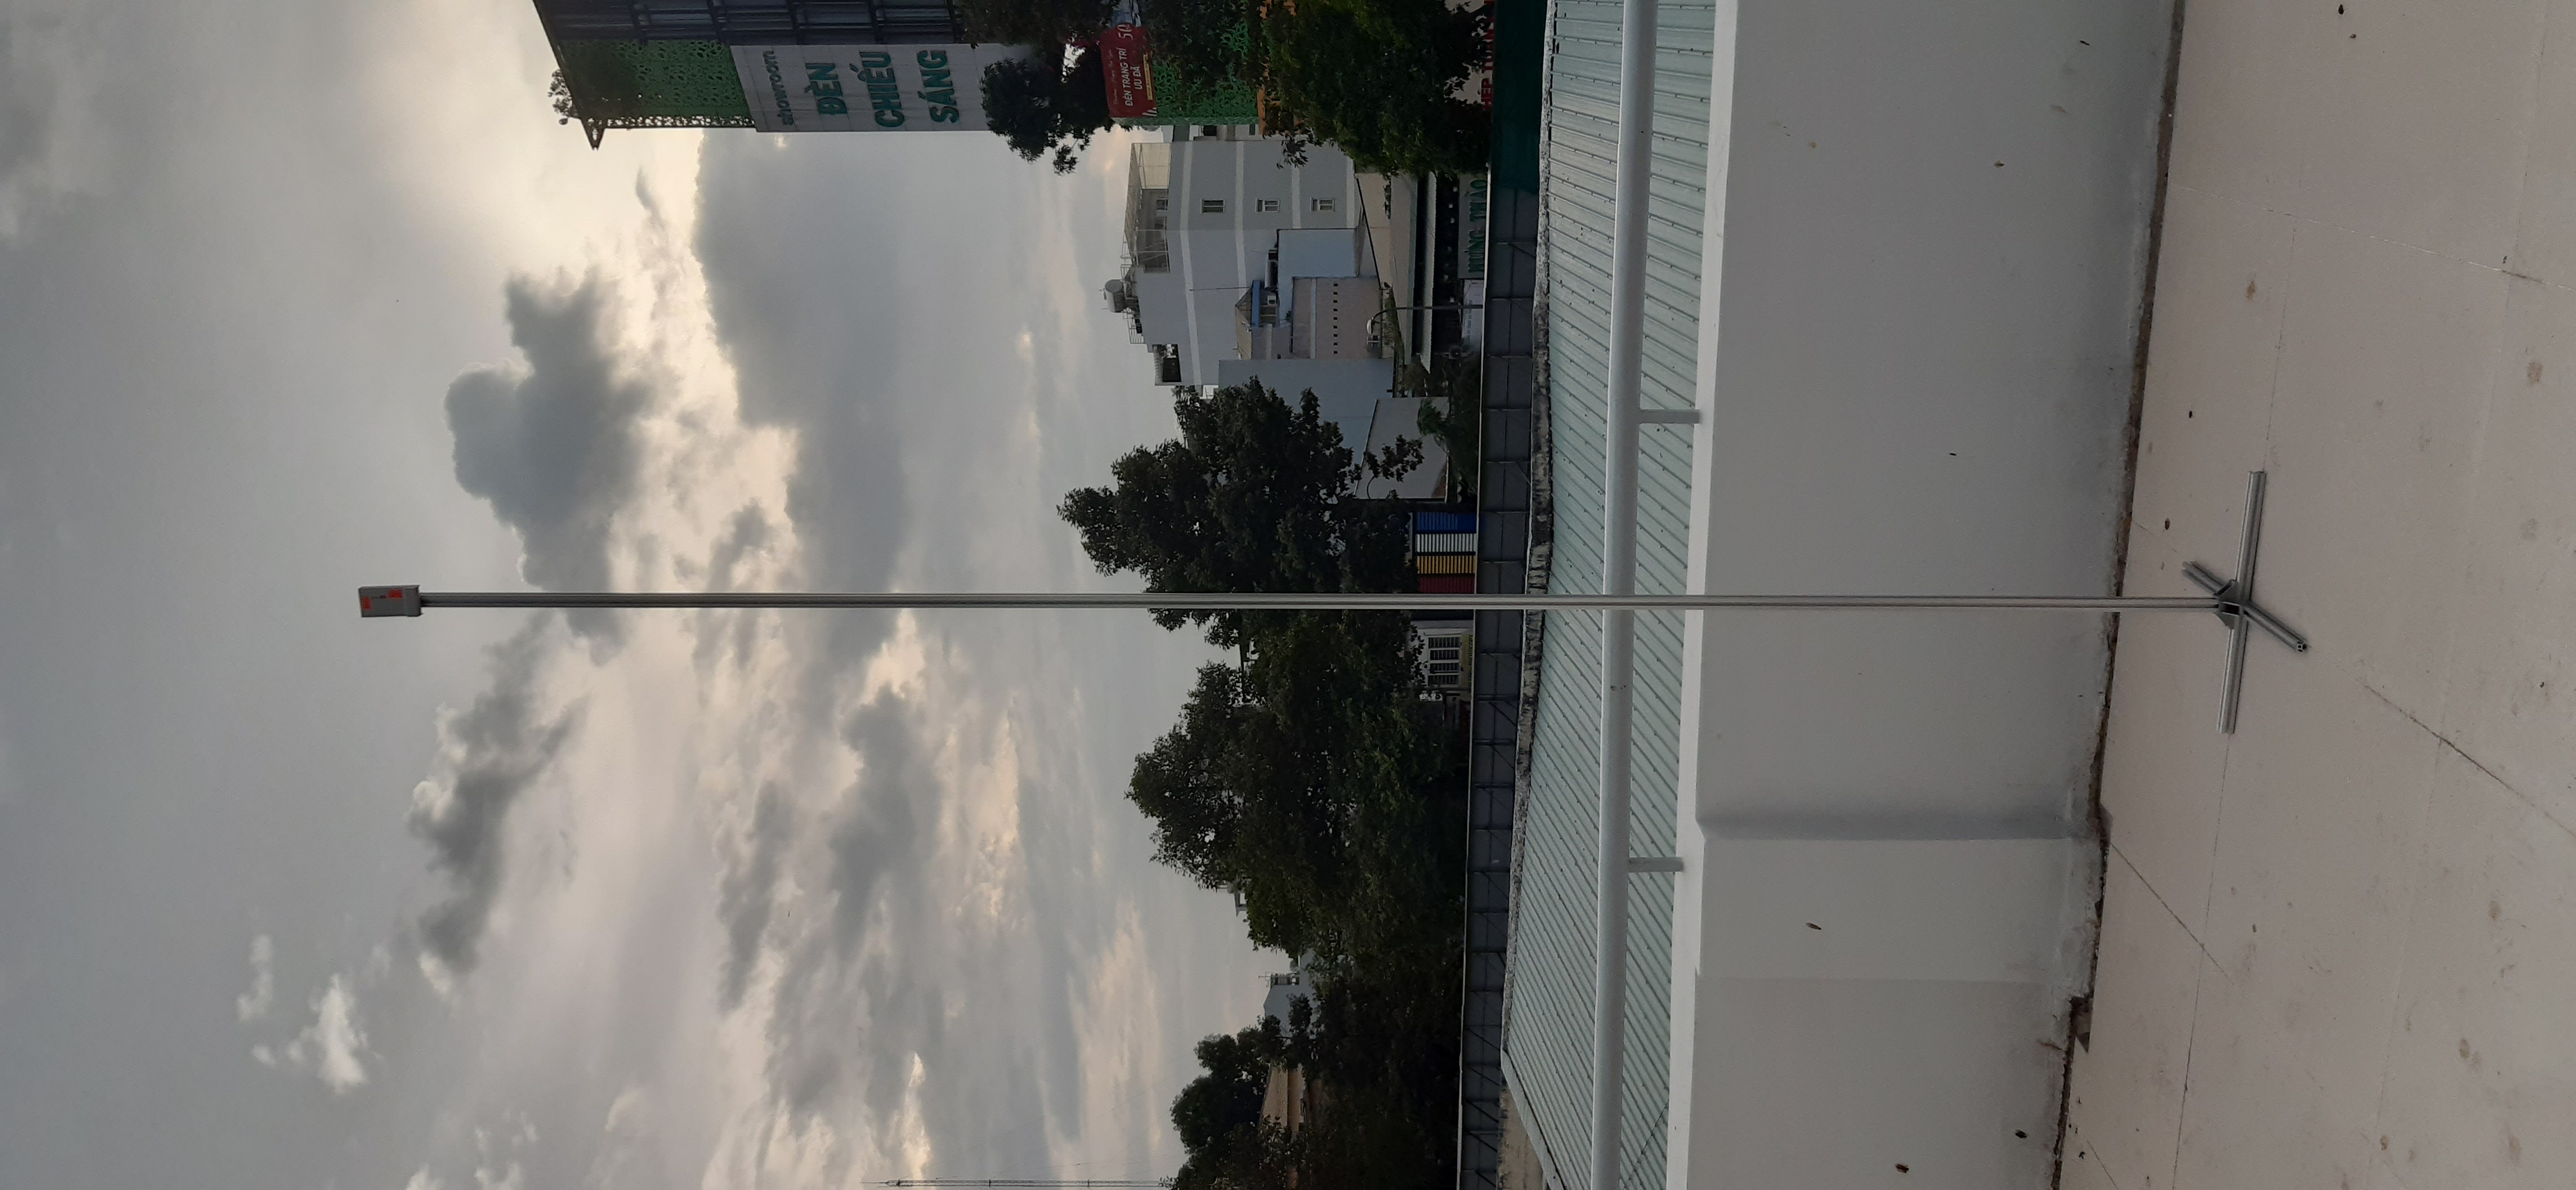
\includegraphics[angle=-90, width=0.65\linewidth]{arena_03.jpg}
%         \label{fig:arena_03}
%     \end{subfigure}
%     \caption{Node 0,1}
%     \label{fig:node_0_1_sep}
% \end{figure}

% \begin{figure}[H]
%     \centering
%     \begin{subfigure}[b]{0.4\linewidth}
%         \centering
%         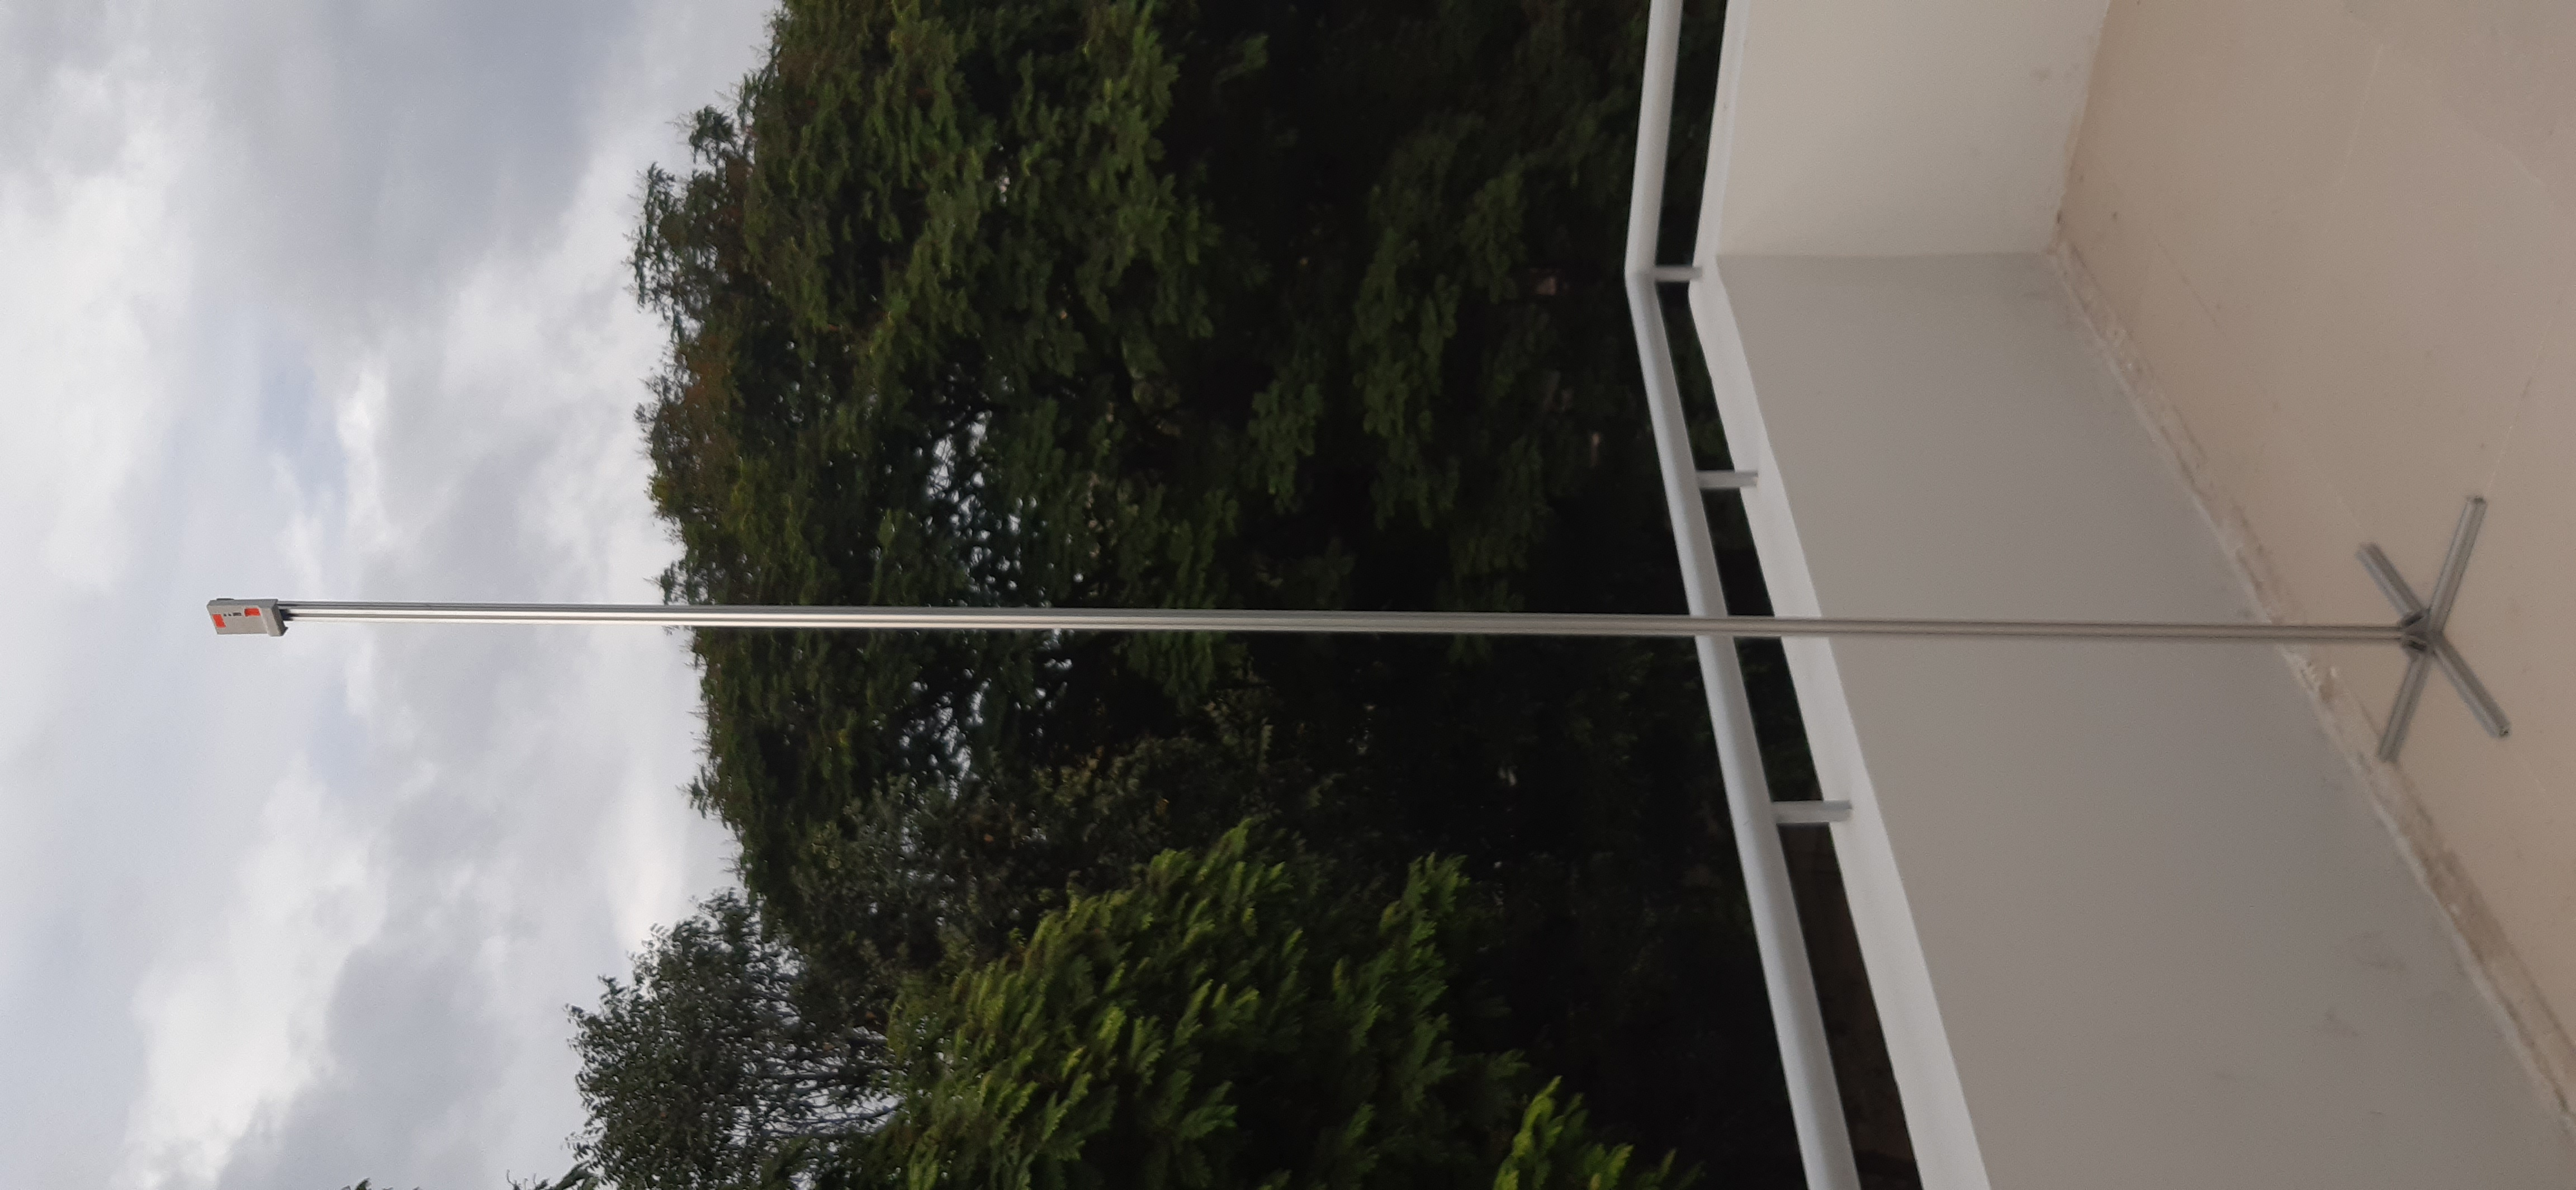
\includegraphics[angle=-90, width=0.65\linewidth]{arena_01.jpg}
%         \label{fig:arena_00}
%     \end{subfigure}
%     \begin{subfigure}[b]{0.4\linewidth}
%         \centering
%         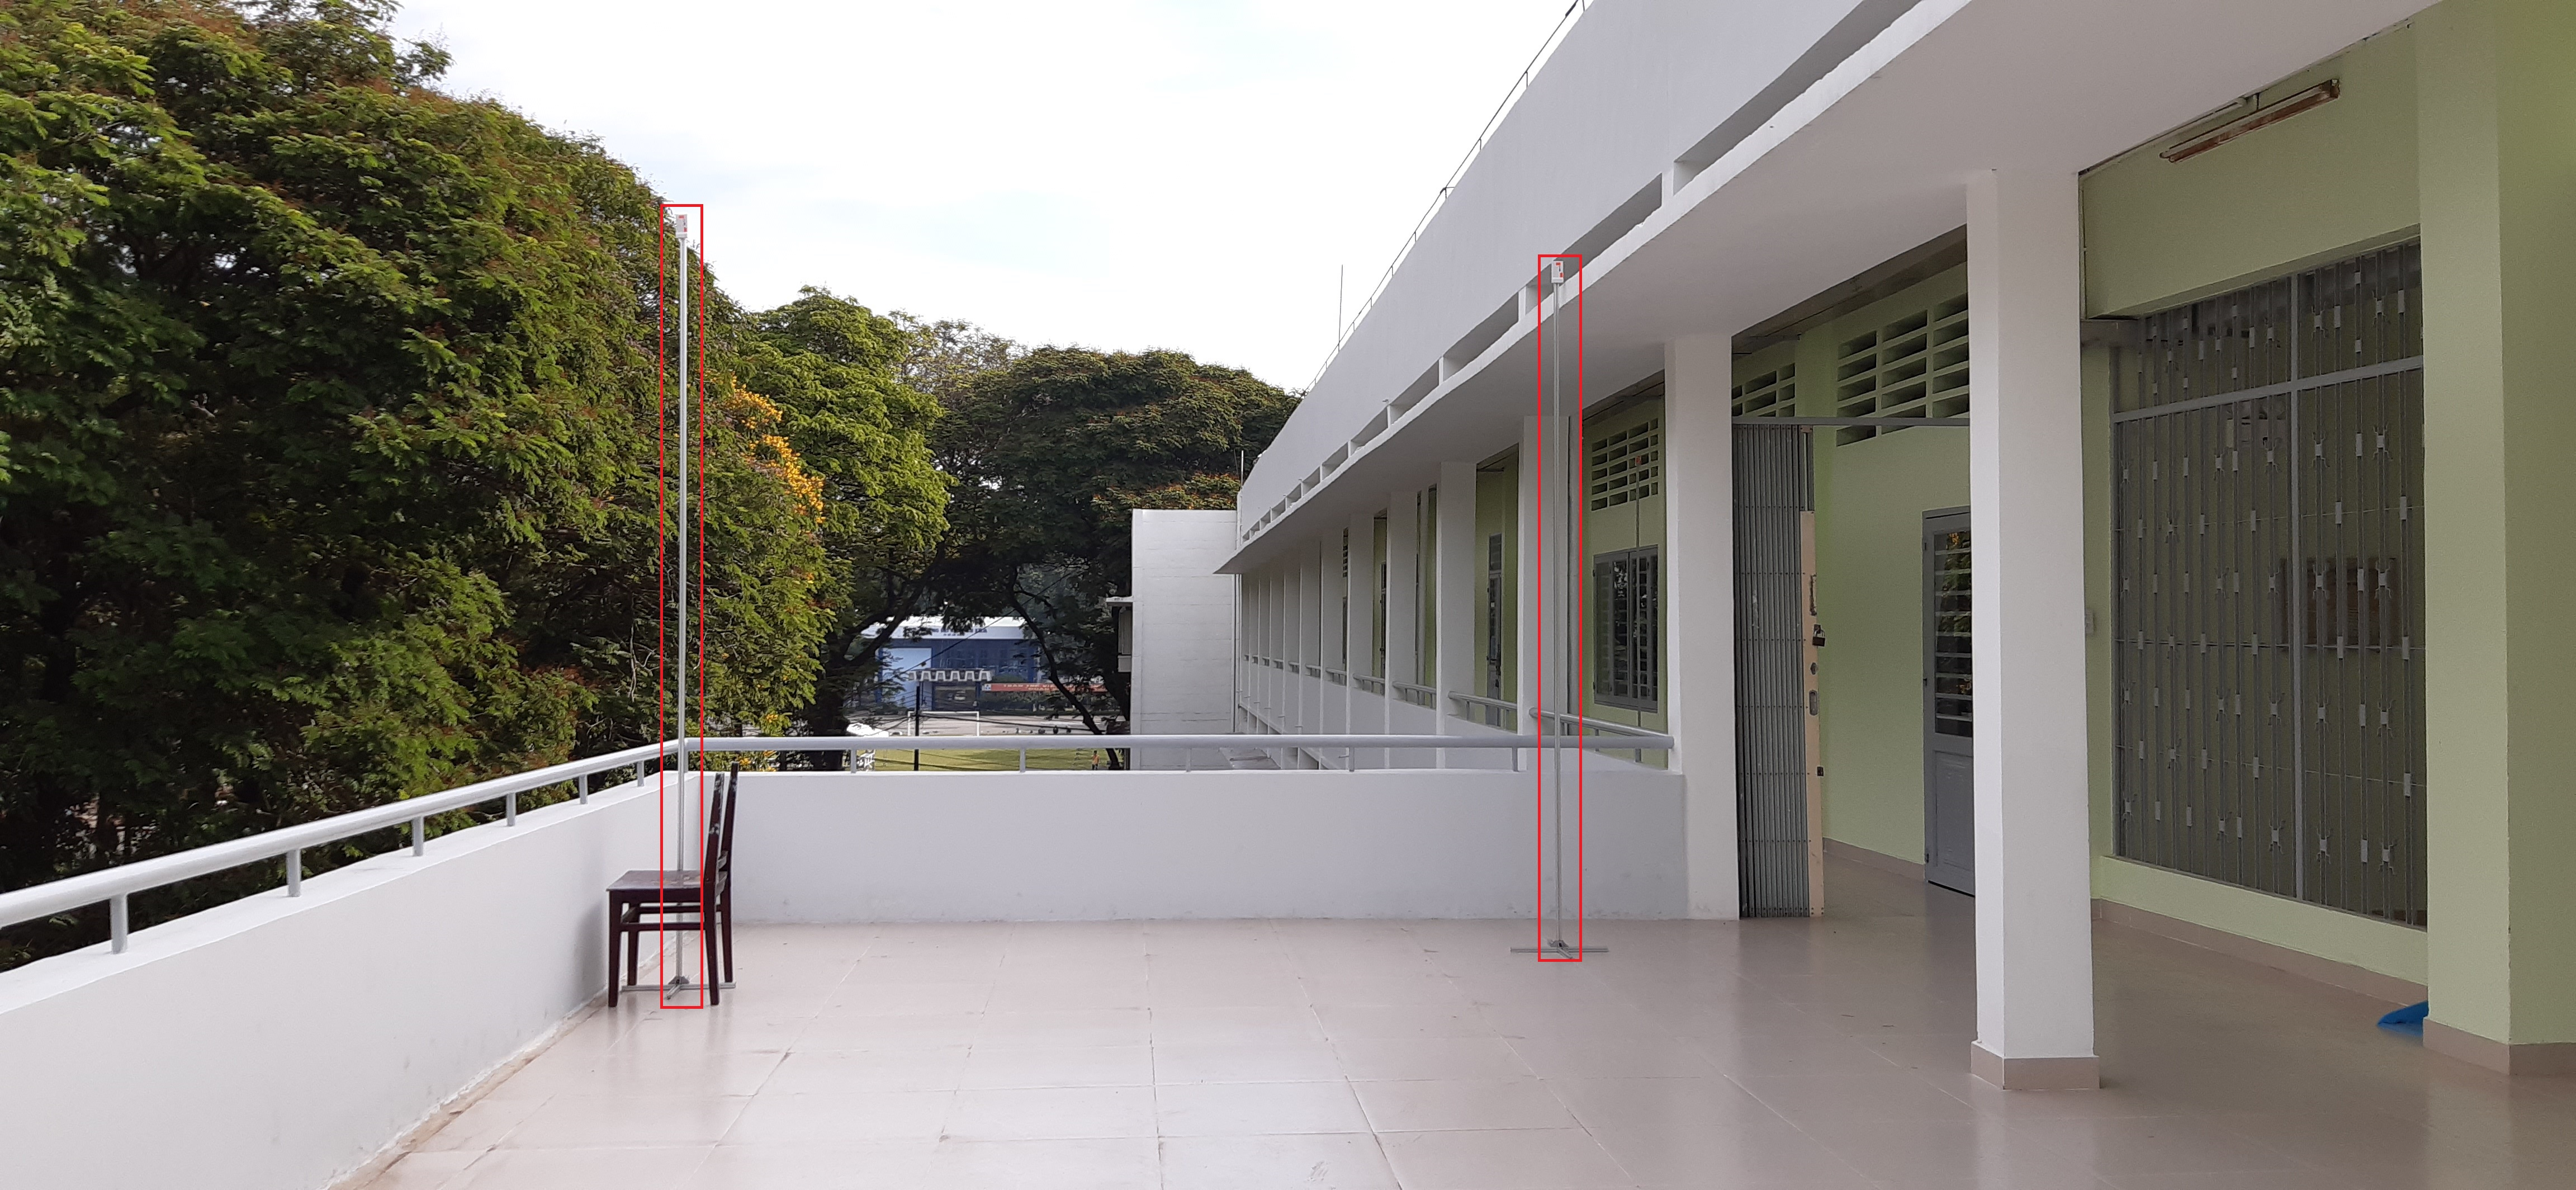
\includegraphics[angle=-90, width=0.65\linewidth]{arena_02.jpg}
%         \label{fig:arena_02}
%     \end{subfigure}
%     \caption{Node 3,4}
%     \label{fig:node_3_4_sep}
% \end{figure}
Results illustrated in figure \ref{fig:multi_cell_movement_result} are obtained as a tag moves along the red line. Since the reference path is not accurate enough, a numeric error is not provided. Notice that red lines are the reference path and blue dots are estimated positions as the tag move along the path.
\begin{figure}[H]
    \centering
    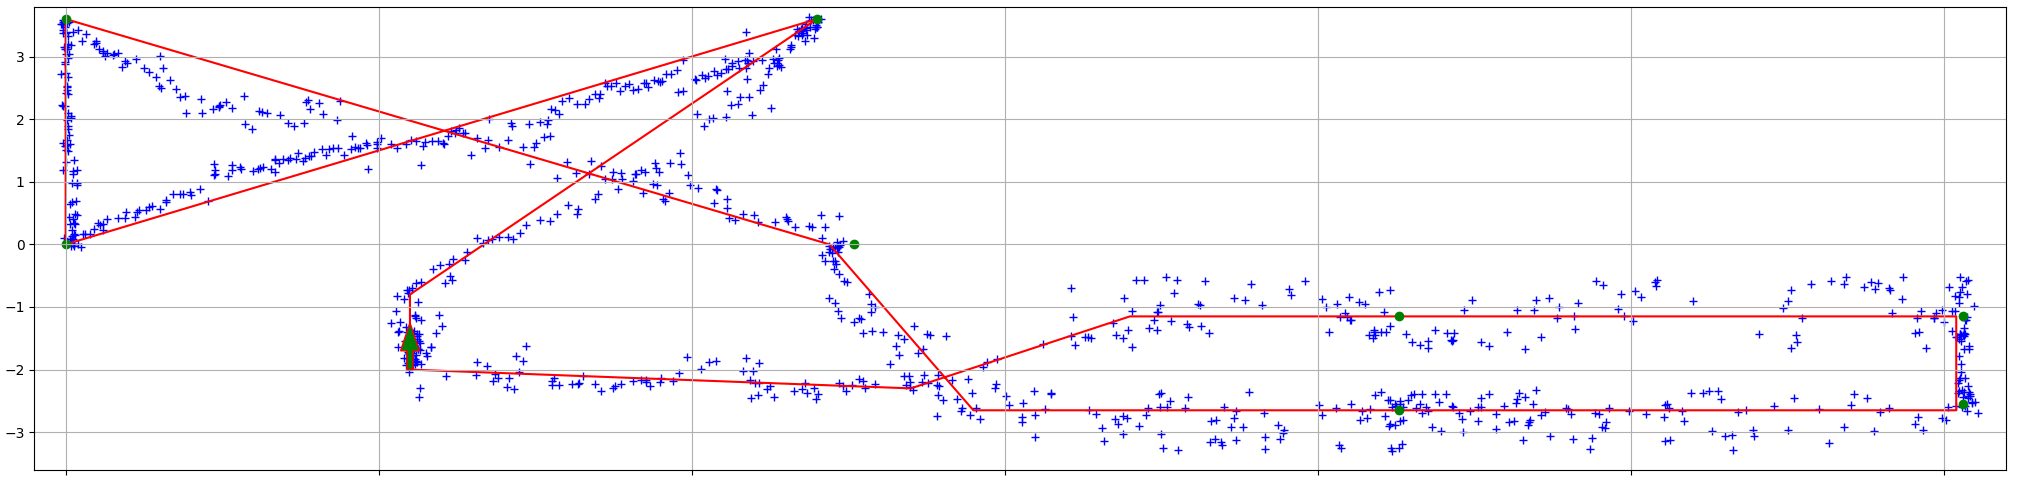
\includegraphics[width=1\textwidth]{path.png}
    \caption{Multi-cell movement result}
    \label{fig:multi_cell_movement_result}
\end{figure}
\subsubsection{Evaluation}
System error increases significantly when anchors are placed to form a narrow shape. Hence, square topology should be used in practice.

\subsection{Scenario 4: IoT Services}
\subsubsection{Objective}
In this thesis, the Bluetooth mesh network is also configured to provide some IoT services. This subsubsection presents the result of remotely controlling the bulb attached to each anchor.
\subsubsection{Result}

Figure \ref{fig:result_remote_control_off_result} illustrated the OFF state of the bulb when receiving OFF messages. As shown in figure \ref{fig:result_remote_control_off_gui}, when a user clicks on the light control button (marked as red number 1), the web socket will publish an ONOFF message with the value of 0 (marked as red number 3). After a while, the GUI receives an ONOFF reply message from the localization system (marked as red number 4) and displays the result using two small light bulb icons (marked as red number 5).

Figure \ref{fig:result_remote_control_on_result} illustrated the ON state of the bulb when receiving ON messages. As shown in figure \ref{fig:result_remote_control_on_gui}, when a user clicks on the light control button (marked as red number 1), the web socket will publish an ONOFF message with the value of 6 (marked as red number 3). After a while, the GUI receives an ONOFF reply message from the localization system (marked as red number 4) and displays the result using two small light bulb icons (marked as red number 5).

\begin{figure}[H]
    \centering
    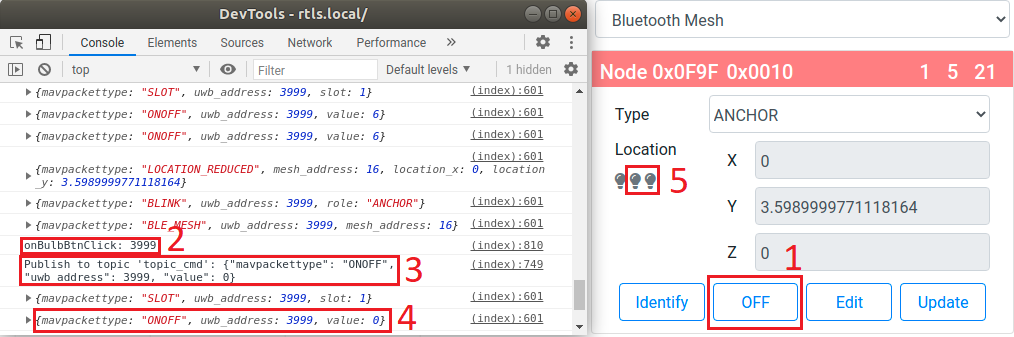
\includegraphics[width=1\textwidth]{result_remote_control_off_gui.png}
    \caption{Control the bulb off}
    \label{fig:result_remote_control_off_gui}
\end{figure}

\begin{figure}[H]
    \centering
    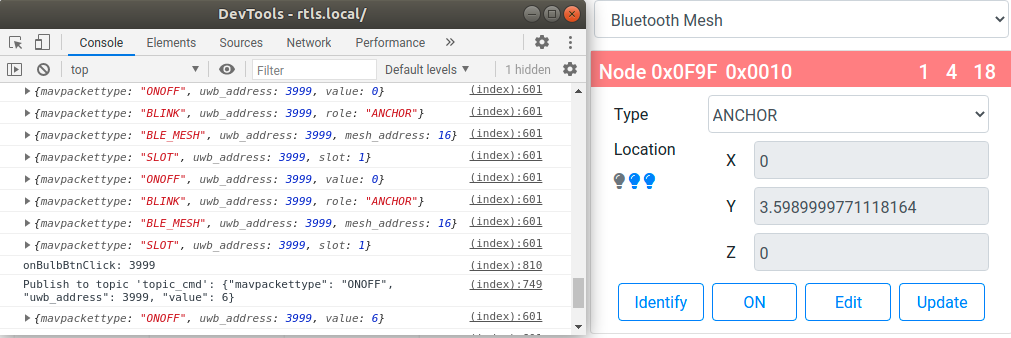
\includegraphics[width=1\textwidth]{result_remote_control_on_gui.png}
    \caption{Control the bulb on}
    \label{fig:result_remote_control_on_gui}
\end{figure}


% \begin{figure}[H]
%     \centering
%     \begin{subfigure}[b]{0.4\linewidth}
%         \centering
%         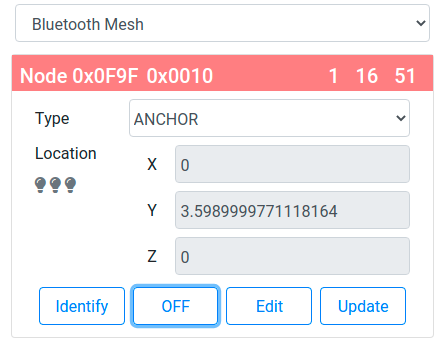
\includegraphics[width=0.9\linewidth]{result_remote_control_off.png}
%         \caption{Bulb off}
%         \label{fig:result_remote_control_off}
%     \end{subfigure}
%     \begin{subfigure}[b]{0.4\linewidth}
%         \centering
%         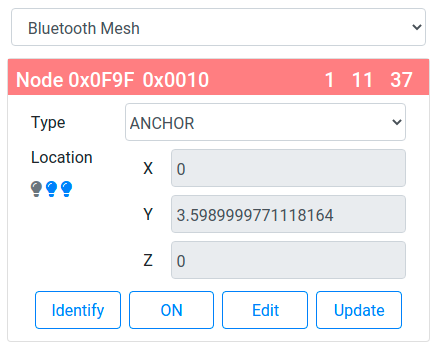
\includegraphics[width=0.9\linewidth]{result_remote_control_on.png}
%         \caption{Bulb on}
%         \label{fig:result_remote_control_on}
%     \end{subfigure}
%     \caption{GUI for remote on-off control}
%     \label{fig:result_remote_control_gui}
% \end{figure}

\begin{figure}[H]
    \centering
    \begin{subfigure}[b]{0.4\linewidth}
        \centering
        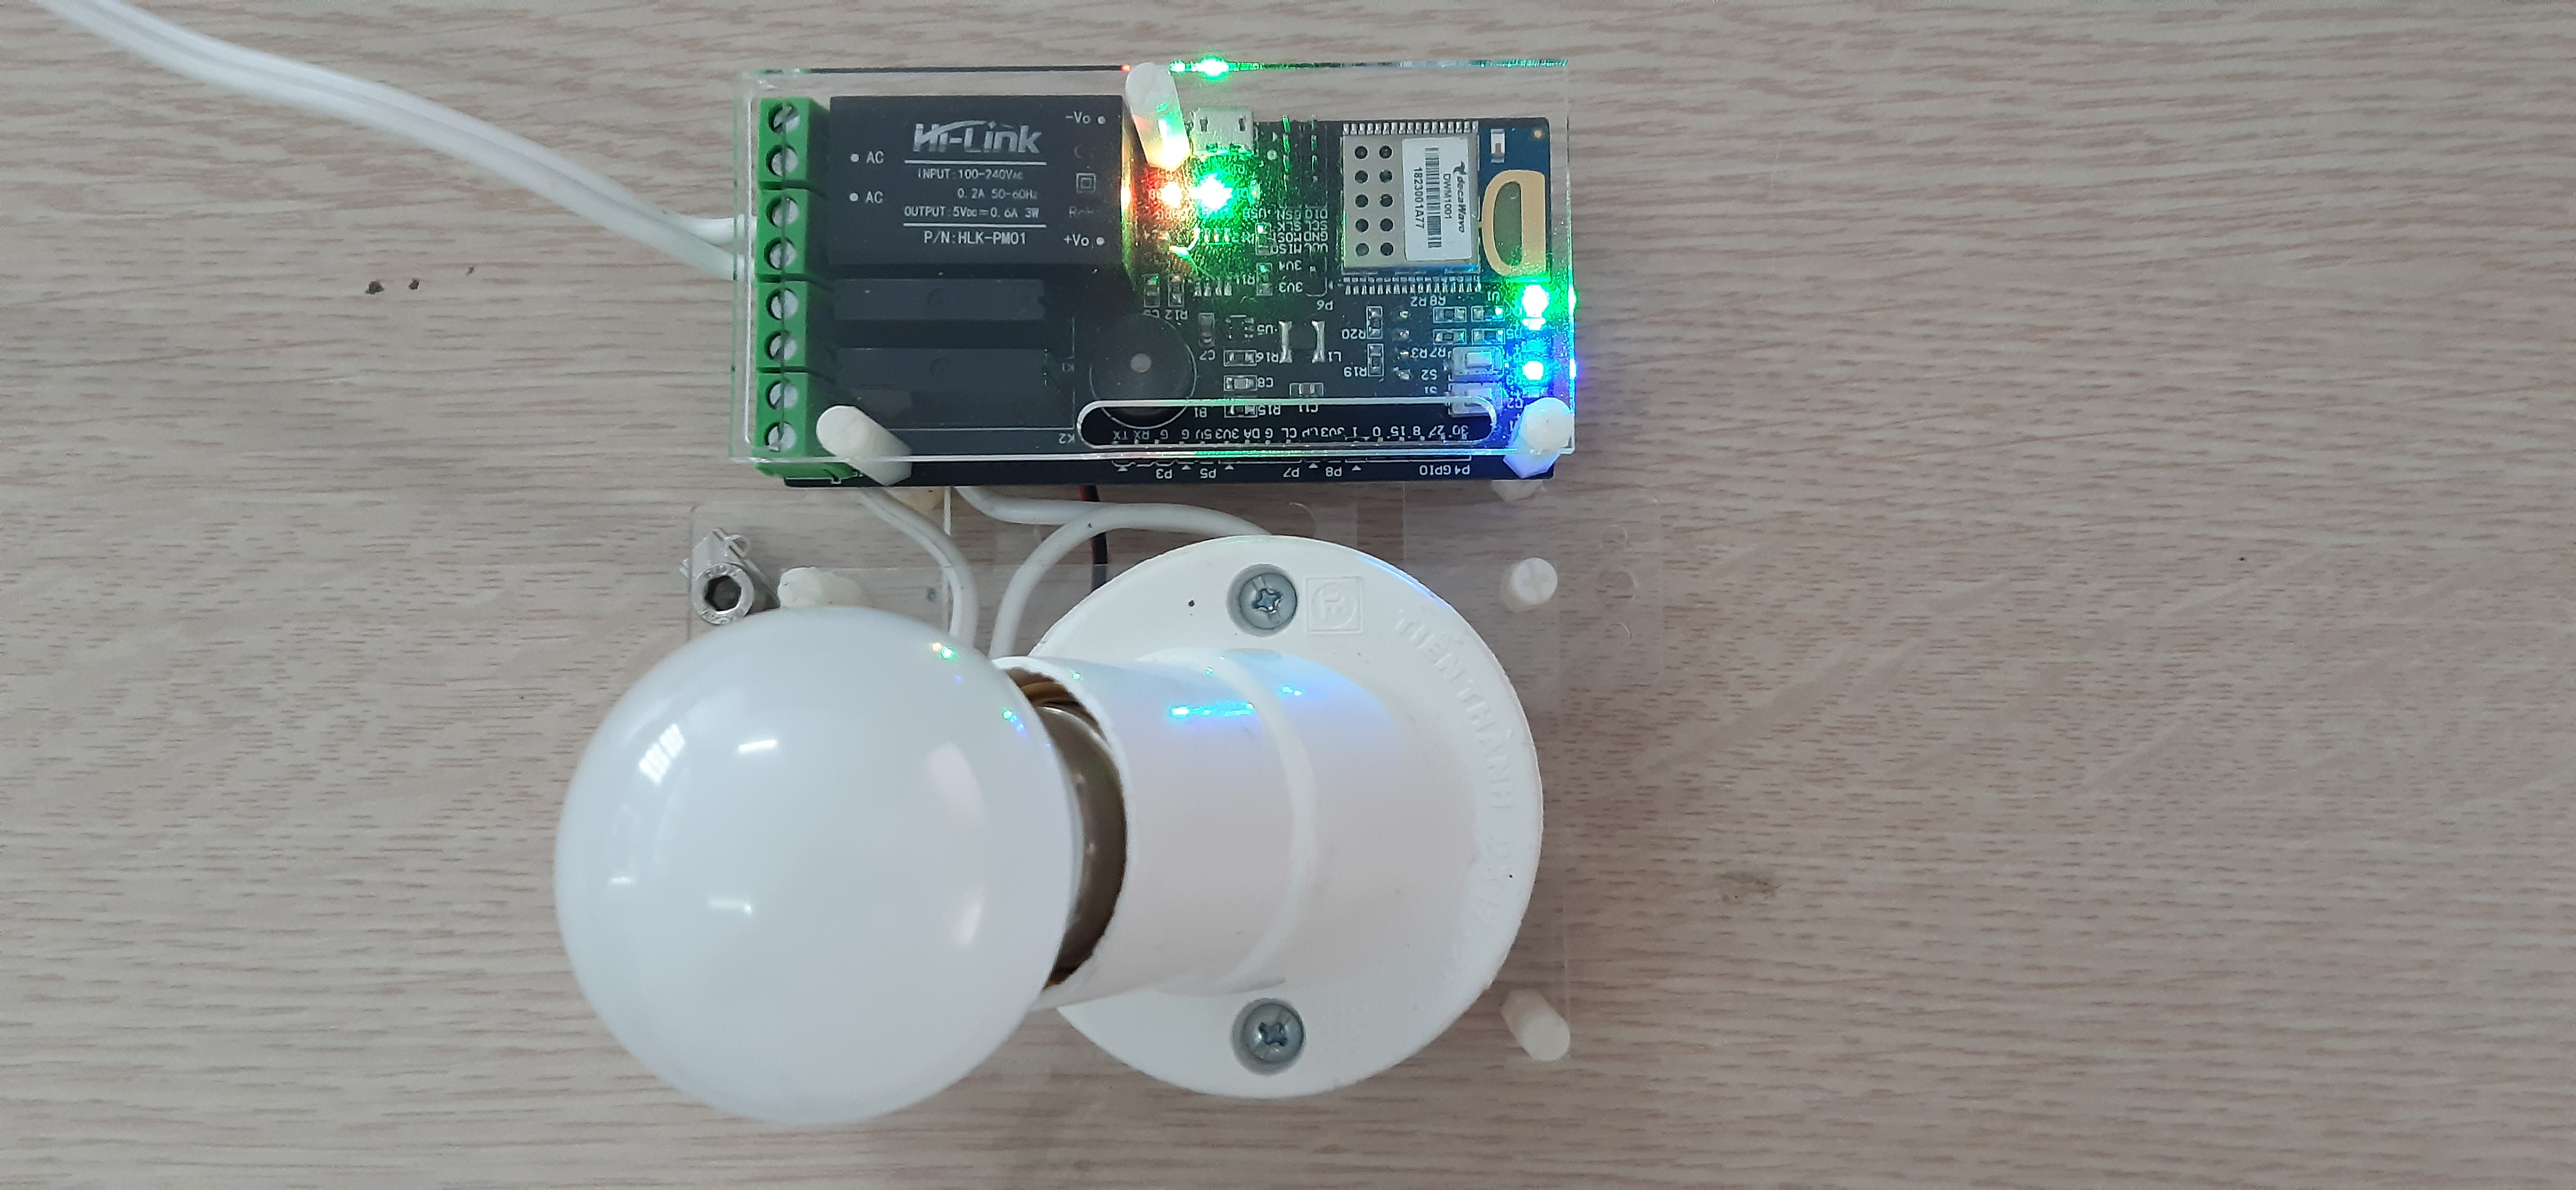
\includegraphics[angle = 90, width=0.9\linewidth]{result_remote_control_off_result.jpg}
        \caption{Bulb off}
        \label{fig:result_remote_control_off_result}
    \end{subfigure}
    \begin{subfigure}[b]{0.4\linewidth}
        \centering
        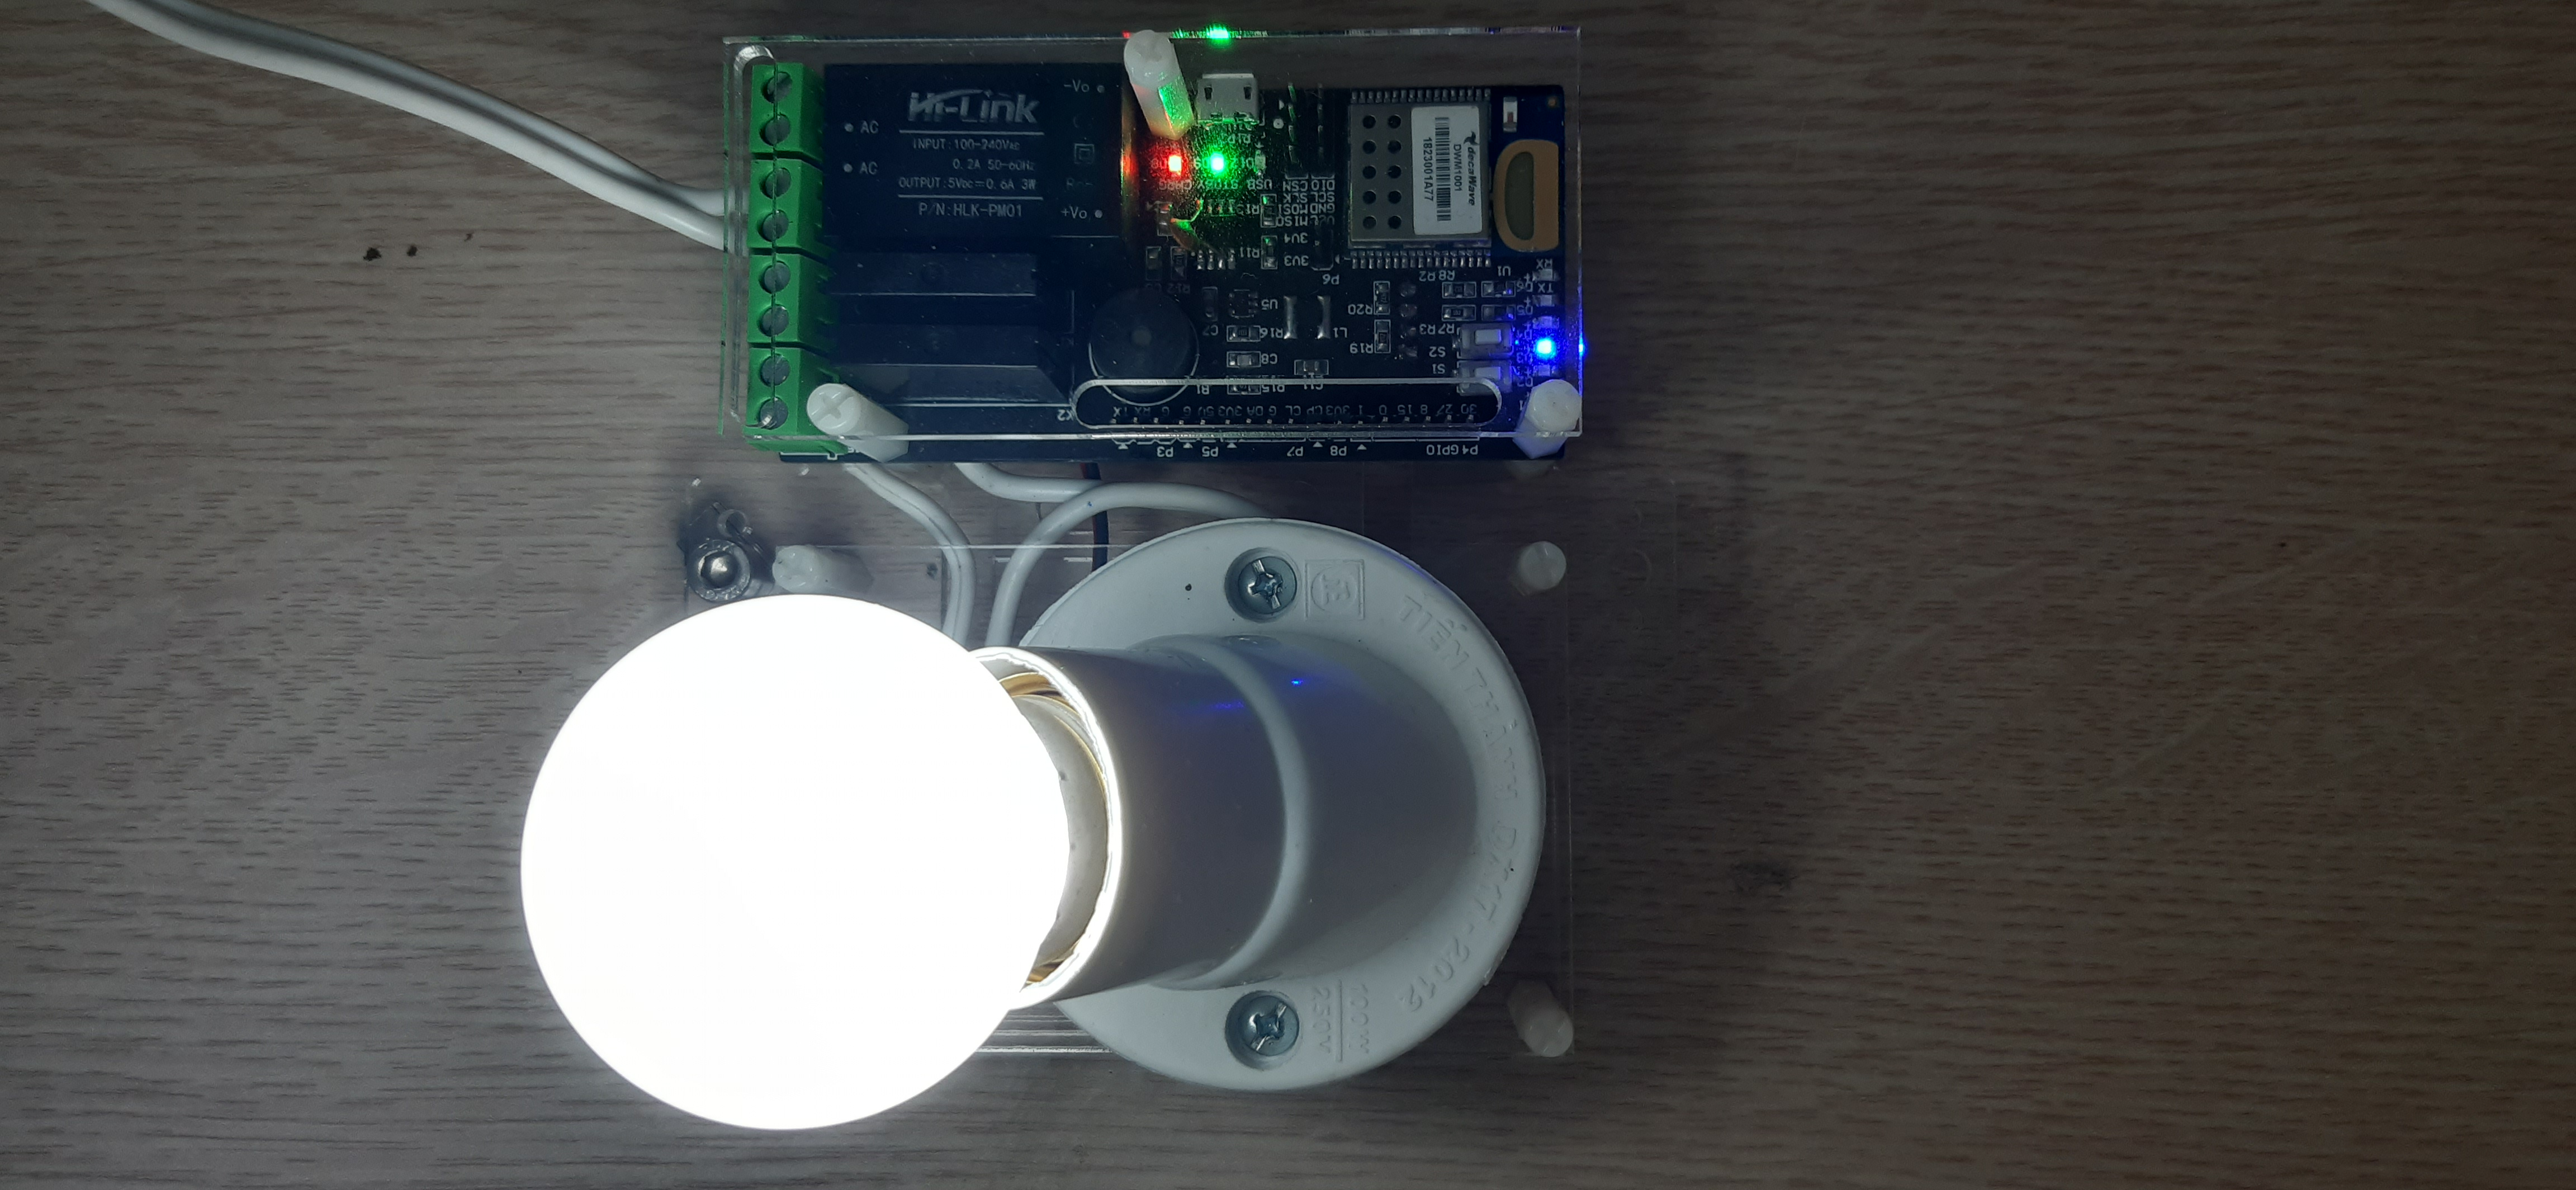
\includegraphics[angle = 90, width=0.9\linewidth]{result_remote_control_on_result.jpg}
        \caption{Bulb on}
        \label{fig:result_remote_control_on_result}
    \end{subfigure}
    \caption{Remote on-off control}
    \label{fig:result_remote_control}
\end{figure}


\subsubsection{Evaluation}
The Bluetooth mesh system has successfully provided remote control service to the system.

\end{document}